%***************************************************************************************************
%***************************************************************************************************
%                                                                                                       
%      Authors: 
%          Marco Buttu, mbuttu@oa-cagliari.inaf.it
%         
%***************************************************************************************************
%***************************************************************************************************
%
\ifx\pdfoutput\undefined
\documentclass[a4paper,12pt,italian]{book}
\else
\documentclass[pdftex,a4paper,12pt,italian]{book}
\fi
%
%***************************************************************************************************
% USEPACKAGE
%***************************************************************************************************
%
\usepackage{fancyhdr}
\usepackage[T1]{fontenc}
\usepackage[italian]{babel}
\usepackage[latin1]{inputenc}
\usepackage[namelimits]{amsmath}
\usepackage{amsfonts,amssymb,amsthm}
\usepackage{makeidx}
\usepackage{index}
\usepackage{color}
\usepackage{subfigure}
\pagestyle{headings}
\usepackage{syntonly}
\usepackage{listings}
\usepackage{multirow}
\usepackage{array}
\usepackage[hang,small,bf]{caption2}
%
%
%********************************
% pdf, ps and  dvi management
%********************************
\ifx\pdfoutput\undefined 
         \usepackage[dvips]{graphicx}
         \RequirePackage[dvipdfm,hyperindex]{hyperref}

         \else
         \usepackage[pdftex]{graphicx}
         \DeclareGraphicsExtensions{.pdf,.png,.jpg,.mps}
	 \usepackage[pdftex,plainpages=false,colorlinks,hyperindex,bookmarksopen,
	 linkcolor=link-color,citecolor=blue,urlcolor=blue]{hyperref}
	 \hypersetup{
         pdftitle={Receiver Library},
         pdfauthor={Marco Buttu},
         }
\fi
%
%***************************************************************************************************
%
\usepackage[cdot,thickqspace,squaren,italian]{SIunits}
%
%***************************************************************************************************
% END USEPACKAGE
%***************************************************************************************************
%
\DeclareMathOperator{\sen}{sen}
\DeclareMathOperator{\arcsen}{arcsen}
%
\newtheorem{esempio}{Esempio}[section]
%
\newcommand{\R}{\mathbb{R}} 
\newcommand{\N}{\mathbb{N}} 
\newcommand{\C}{\mathbb{C}} 
\newcommand{\Z}{\mathbb{Z}} 
%
\newcommand{\drt}{derotator}
%
\newcommand{\di}{\mathrm{d}}
\providecommand{\abs}[1]{\lvert#1\rvert}
%
\definecolor{mygray}{rgb}{0.9,0.9,0.9}
\definecolor{mygreen}{rgb}{0,0.6,0}
\definecolor{myblue}{rgb}{0,0,1}
\definecolor{darkred}{rgb}{0.5,0,0}
\definecolor{mylightblue}{rgb}{0,0,0.7}
\definecolor{stringa}{rgb}{1,0.1,0}
\definecolor{sfondo_sorgente}{rgb}{0.95,0.95,0.95}
\definecolor{mykey}{rgb}{0.7,0.4,0}
\definecolor{link-color}{rgb}{0.74,0.12,0}
\definecolor{sfondo_shell}{rgb}{0.90,0.90,0.70}
%
%
\interfootnotelinepenalty=10000 % footnote su unica pagina 
%
%
%***************************************************************************************************
% LISTINGS
%***************************************************************************************************
%
\renewcommand{\lstlistlistingname}{Elenco dei listati}% toc dei listati
\renewcommand{\lstlistingname}{Listato}% nome nella caption
\lstset{
 language=verilog, 
 basicstyle=\small\ttfamily,
 keywordstyle=\color{myblue}\small\ttfamily,
 emph={module,endmodule},
 emphstyle=\color{black}\small\bfseries\sffamily,
 emph={[2] finish, monitor, time},
 emphstyle={[2]\color{mykey}\small\ttfamily},
 emph={[3] timescale},
 emphstyle={[3]\color{stringa}\small\ttfamily},
 emphstyle={[4]\color{black}\small\ttfamily},
 stringstyle=\ttfamily,
 showstringspaces=false,
 captionpos=b,
 belowcaptionskip=10pt,
 columns=flexible,
 aboveskip=10pt,
 backgroundcolor=\color{sfondo_sorgente},
 frame=single,
 framerule=0pt,  % rettandolo racchiuso da una linea spessa 0pt
 tabsize=2,
 %numbers=left,numberstyle={\scriptsize}, stepnumber=1, numbersep=10pt,
 %numberstyle=\tiny,
 framexleftmargin=1mm,
 framexrightmargin=1mm,
 commentstyle=\color{mygreen}\ttfamily, % mygreen comments
 extendedchars=true,  % abilito l'utilizzo dei caratteri nazionali ( �, �, ecc. )
 literate=%
 {'b}{{'{\color{red}b}}}1
 {'h}{{'{\color{red}h}}}1
 {'d}{{'{\color{red}d}}}1
%
 {0]}{{{\color{red}0}]}}1
 {1]}{{{\color{red}1}]}}1
 {2]}{{{\color{red}2}]}}1
 {3]}{{{\color{red}3}]}}1
 {4]}{{{\color{red}4}]}}1
 {5]}{{{\color{red}5}]}}1
 {6]}{{{\color{red}6}]}}1
 {7]}{{{\color{red}7}]}}1
 {8]}{{{\color{red}8}]}}1
 {9]}{{{\color{red}9}]}}1
%
 {:0}{{:{\color{red}0}}}1
 {:1}{{:{\color{red}1}}}1
 {:2}{{:{\color{red}2}}}1
 {:3}{{:{\color{red}3}}}1
 {:4}{{:{\color{red}4}}}1
 {:5}{{:{\color{red}5}}}1
 {:6}{{:{\color{red}6}}}1
 {:7}{{:{\color{red}7}}}1
 {:8}{{:{\color{red}8}}}1
 {:9}{{:{\color{red}9}}}1
%
 {-0:}{{-{\color{red}0}:}}1
 {-1:}{{-{\color{red}1}:}}1
 {-2:}{{-{\color{red}2}:}}1
 {-3:}{{-{\color{red}3}:}}1
 {-4:}{{-{\color{red}4}:}}1
 {-5:}{{-{\color{red}5}:}}1
 {-6:}{{-{\color{red}6}:}}1
 {-7:}{{-{\color{red}7}:}}1
 {-8:}{{-{\color{red}8}:}}1
 {-9:}{{-{\color{red}9}:}}1
%
 {0:}{{{\color{red}0}:}}1
 {1:}{{{\color{red}1}:}}1
 {2:}{{{\color{red}2}:}}1
 {3:}{{{\color{red}3}:}}1
 {4:}{{{\color{red}4}:}}1
 {5:}{{{\color{red}5}:}}1
 {6:}{{{\color{red}6}:}}1
 {7:}{{{\color{red}7}:}}1
 {8:}{{{\color{red}8}:}}1
 {9:}{{{\color{red}9}:}}1
%
 {0: }{{{\color{black}0}:}}1
 {1: }{{{\color{black}1}:}}1
 {2: }{{{\color{black}2}:}}1
 {3: }{{{\color{black}3}:}}1
 {4: }{{{\color{black}4}:}}1
 {5: }{{{\color{black}5}:}}1
 {6: }{{{\color{black}6}:}}1
 {7: }{{{\color{black}7}:}}1
 {8: }{{{\color{black}8}:}}1
 {9: }{{{\color{black}9}:}}1
 %
 {0*}{{{\color{red}0}*}}1
 {1*}{{{\color{red}1}*}}1
 {2*}{{{\color{red}2}*}}1
 {3*}{{{\color{red}3}*}}1
 {4*}{{{\color{red}4}*}}1
 {5*}{{{\color{red}5}*}}1
 {6*}{{{\color{red}6}*}}1
 {7*}{{{\color{red}7}*}}1
 {8*}{{{\color{red}8}*}}1
 {9*}{{{\color{red}9}*}}1
%
 {[0}{{[{\color{red}0}}}1
 {[1}{{[{\color{red}1}}}1
 {[2}{{[{\color{red}2}}}1
 {[3}{{[{\color{red}3}}}1
 {[4}{{[{\color{red}4}}}1
 {[5}{{[{\color{red}5}}}1
 {[6}{{[{\color{red}6}}}1
 {[7}{{[{\color{red}7}}}1
 {[8}{{[{\color{red}8}}}1
 {[9}{{[{\color{red}9}}}1
 %
 {\_0]}{{\_{\color{black}0}]}}1
 {\_1]}{{\_{\color{black}1}]}}1
 {\_2]}{{\_{\color{black}2}]}}1
 {\_3]}{{\_{\color{black}3}]}}1
 {\_4]}{{\_{\color{black}4}]}}1
 {\_5]}{{\_{\color{black}5}]}}1
 {\_6]}{{\_{\color{black}6}]}}1
 {\_7]}{{\_{\color{black}7}]}}1
 {\_8]}{{\_{\color{black}8}]}}1
 {\_9]}{{\_{\color{black}9}]}}1
}
\lstset{morecomment=[s][\color{stringa}]{"}{"}}
\lstset{morecomment=[l][\color{myblue}]{\#}}
%
%
\lstdefinestyle{output}{
 basicstyle=\small\ttfamily,
 showstringspaces=false,
 captionpos=b,
 belowcaptionskip=10pt,
 columns=flexible,
 aboveskip=10pt,
 framexleftmargin=3mm, 
 framexrightmargin=2mm,
 frame=shadowbox, 
 rulesepcolor=\color{black}, 
 backgroundcolor=\color{white}, 
 framerule=1pt,
 tabsize=2,
 literate=%
 {'b}{{'{\color{red}b}}}1
 {'h}{{'{\color{red}h}}}1
 {'d}{{'{\color{red}d}}}1
%
 {0]}{{{\color{red}0}]}}1
 {1]}{{{\color{red}1}]}}1
 {2]}{{{\color{red}2}]}}1
 {3]}{{{\color{red}3}]}}1
 {4]}{{{\color{red}4}]}}1
 {5]}{{{\color{red}5}]}}1
 {6]}{{{\color{red}6}]}}1
 {7]}{{{\color{red}7}]}}1
 {8]}{{{\color{red}8}]}}1
 {9]}{{{\color{red}9}]}}1
%
 {:0}{{:{\color{red}0}}}1
 {:1}{{:{\color{red}1}}}1
 {:2}{{:{\color{red}2}}}1
 {:3}{{:{\color{red}3}}}1
 {:4}{{:{\color{red}4}}}1
 {:5}{{:{\color{red}5}}}1
 {:6}{{:{\color{red}6}}}1
 {:7}{{:{\color{red}7}}}1
 {:8}{{:{\color{red}8}}}1
 {:9}{{:{\color{red}9}}}1
%
 {-0:}{{-{\color{red}0}:}}1
 {-1:}{{-{\color{red}1}:}}1
 {-2:}{{-{\color{red}2}:}}1
 {-3:}{{-{\color{red}3}:}}1
 {-4:}{{-{\color{red}4}:}}1
 {-5:}{{-{\color{red}5}:}}1
 {-6:}{{-{\color{red}6}:}}1
 {-7:}{{-{\color{red}7}:}}1
 {-8:}{{-{\color{red}8}:}}1
 {-9:}{{-{\color{red}9}:}}1
%
 {0:}{{{\color{red}0}:}}1
 {1:}{{{\color{red}1}:}}1
 {2:}{{{\color{red}2}:}}1
 {3:}{{{\color{red}3}:}}1
 {4:}{{{\color{red}4}:}}1
 {5:}{{{\color{red}5}:}}1
 {6:}{{{\color{red}6}:}}1
 {7:}{{{\color{red}7}:}}1
 {8:}{{{\color{red}8}:}}1
 {9:}{{{\color{red}9}:}}1
%
 {0: }{{{\color{black}0}:}}1
 {1: }{{{\color{black}1}:}}1
 {2: }{{{\color{black}2}:}}1
 {3: }{{{\color{black}3}:}}1
 {4: }{{{\color{black}4}:}}1
 {5: }{{{\color{black}5}:}}1
 {6: }{{{\color{black}6}:}}1
 {7: }{{{\color{black}7}:}}1
 {8: }{{{\color{black}8}:}}1
 {9: }{{{\color{black}9}:}}1
 %
 {0*}{{{\color{red}0}*}}1
 {1*}{{{\color{red}1}*}}1
 {2*}{{{\color{red}2}*}}1
 {3*}{{{\color{red}3}*}}1
 {4*}{{{\color{red}4}*}}1
 {5*}{{{\color{red}5}*}}1
 {6*}{{{\color{red}6}*}}1
 {7*}{{{\color{red}7}*}}1
 {8*}{{{\color{red}8}*}}1
 {9*}{{{\color{red}9}*}}1
%
 {[0}{{[{\color{red}0}}}1
 {[1}{{[{\color{red}1}}}1
 {[2}{{[{\color{red}2}}}1
 {[3}{{[{\color{red}3}}}1
 {[4}{{[{\color{red}4}}}1
 {[5}{{[{\color{red}5}}}1
 {[6}{{[{\color{red}6}}}1
 {[7}{{[{\color{red}7}}}1
 {[8}{{[{\color{red}8}}}1
 {[9}{{[{\color{red}9}}}1
 %
 {\_0]}{{\_{\color{black}0}]}}1
 {\_1]}{{\_{\color{black}1}]}}1
 {\_2]}{{\_{\color{black}2}]}}1
 {\_3]}{{\_{\color{black}3}]}}1
 {\_4]}{{\_{\color{black}4}]}}1
 {\_5]}{{\_{\color{black}5}]}}1
 {\_6]}{{\_{\color{black}6}]}}1
 {\_7]}{{\_{\color{black}7}]}}1
 {\_8]}{{\_{\color{black}8}]}}1
 {\_9]}{{\_{\color{black}9}]}}1
 }
%
\lstset{
language=C++,
 basicstyle=\small\ttfamily,
 keywordstyle=\color{myblue}\small\ttfamily,
 emphstyle=\color{black}\small\bfseries\sffamily,
 emph={[2] finish, monitor, time},
 emphstyle={[2]\color{mykey}\small\ttfamily},
 emph={[3] timescale},
 emphstyle={[3]\color{stringa}\small\ttfamily},
 emphstyle={[5]\color{myblue}\small\ttfamily},
 stringstyle=\ttfamily,
 showstringspaces=false,
 captionpos=b,
 belowcaptionskip=10pt,
 columns=flexible,
 aboveskip=10pt,
 backgroundcolor=\color{sfondo_sorgente},
 frame=single,
 framerule=0pt,  % rettandolo racchiuso da una linea spessa 0pt
 tabsize=2,
 %numbers=left,numberstyle={\scriptsize}, stepnumber=1, numbersep=10pt,
 %numberstyle=\tiny,
 framexleftmargin=1mm,
 framexrightmargin=1mm,
 commentstyle=\color{mygreen}\ttfamily, % mygreen comments
 extendedchars=true,  % abilito l'utilizzo dei caratteri nazionali ( �, �, ecc. )
}
\lstset{morecomment=[s][\color{stringa}]{"}{"}}
\lstset{morecomment=[l][\color{myblue}]{\#}}
%
%***************************************************************************************************
% END LISTINGS
%***************************************************************************************************
%
%
%***************************************************************************************************
% CAPTION2
%***************************************************************************************************
%
\newcommand{\figurecaption}{%
\setlength{\abovecaptionskip}{0pt}
\setlength{\belowcaptionskip}{0pt}
\caption%
}
%
%***************************************************************************************************
% END CAPTION2
%***************************************************************************************************
%
%
%***************************************************************************************************
% INDEX
%***************************************************************************************************
%
\addto\captionsitalian{\def\indexname{Indice analitico}}
%
\makeindex
%
\renewindex{default}{idx}{ind}{\indexname} %equivalent to \makeindex
\newindex{aut}{adx}{and}{Indice dei nomi} % \index[aut]{Marco Buttu}
%
%% latex receiver_library.tex
%% makeindex receiver_library.idx -s index.sty
%% latex receiver_library.tex
%
%
%***************************************************************************************************
% END INDEX
%***************************************************************************************************
%
%
%
%****************************************************************************************
%***************************************************************************************************
% DOCUMENT
%***************************************************************************************************
%****************************************************************************************
%
\begin{document}
\SIunits
%
%***************************************************************************************************
% COVER
%***************************************************************************************************
%
\begin{titlepage}
\thispagestyle{empty}
\begin{center}
Istituto Nazionale di Astrofisica
\\
Osservatorio Astronomico di Cagliari
\\
Localit� Poggio dei Pini, Strada 54, 09012 Capoterra (CA) - Italy
\\
\end{center}
%\begin{flushright}
\begin{center}
\vspace{3cm}
{
\Huge \textsc{\textbf{RECEIVER LIBRARY}}% prima parte del titolo
\\
\rule{\textwidth}{1.5mm}}
\\
\vspace{0.2cm}
\textsc{\small Hardware + Protocol + LNAs and Dewar control library}
\end{center}
% \end{flushright}
\vspace{1cm} % nel caso si inserisca l'immagine
  \begin{center}
   % \includegraphics[width=13.5cm]{figure/dinamica} 
  \end{center}
\vspace{5cm}
\begin{flushright}
Autore: \textbf{Marco Buttu}\\
Email: \texttt{mbuttu@oa-cagliari.inaf.it} \\
Versione 1.0.1, \today
\end{flushright}
\end{titlepage}
%
%***************************************************************************************************
% END COVER
%***************************************************************************************************
%
%
\newpage
\thispagestyle{empty}
\null
%
\thispagestyle{empty}  % elimina intestazione e pi� di pagina
\cleardoublepage
%
{\small \begin{flushleft}\textbf{Receiver Library: Hardware, Protocol, LNAs and Dewar control\\}
Marco Buttu <\texttt{mbuttu@oa-cagliari.inaf.it}>
\end{flushleft}}
\vspace{1cm}

{\small
Questo documento descrive come avviene il controllo dei ricevitori mediante le librerie
\texttt{MicroControllerBoard} e \texttt{ReceiverControl}. Tali librerie possono essere utilizzate
solo per controllare i ricevitori nei queli sono montate le schede a microcontrollore sviluppate
nella Stazione Radioastronomica di Medicina (BO);
Questi ricevitori ospiteranno due schede: una per
il \textbf{controllo del dewar} e una per il \textbf{controllo degli LNA}.

Il protocollo di comunicazione con le schede a microcontrollore \`e descritto nel documento interno 
IRA n.358/04 (F.Fiocchi, G.Macaferri, A.Oralti, M.Morsiani). Il firmware installato nelle schede \`e stato 
realizzato da Franco Fiocchi mentre per i dettagli sull'hardware ci si pu\`o rivolgere a Sandro Cattani
ed Andrea Maccaferri.

Le librerie \texttt{MicroControllerBoard} e \texttt{ReceiverControl}, che permettono di comunicare
con le schede sono state realizzate da Marco Buttu ed Andrea Orlati, e si dispongono su due livelli 
indipendenti: un primo livello (\texttt{MicroControllerBoard}) che fornisce
un'interfaccia per la comunicazione con le schede (sostanziamente un'implementazione del protocollo di
comunicazione), ed un secondo e pi\`u alto livello (\texttt{ReceiverControl}) che mediante l'utilizzo 
della prima libreria definisce una interfaccia per la comunicazione con il ricevitore.
}
\\\vspace{1.5cm}
{\small 
\begin{flushleft}\textbf{Contatti\\}\end{flushleft}
}
{\small
\begin{flushleft}
Per quanto riguarda la parte \textbf{software}:\\
Marco Buttu <\texttt{mbuttu@oa-cagliari.inaf.it}> \\
Andrea Orlati <\texttt{a.orlati@ira.inaf.it}>\\\vspace{0.3cm}
Per il \textbf{firmware}:\\
Franco Fiocchi <\texttt{f.fiocchi@ira.inaf.it}>\\\vspace{0.3cm}
Per quanto riguarda la parte \textbf{hardware}:\\
Sandro Cattani <\texttt{a.cattani@ira.inaf.it}>\\
Andrea Maccaferri <\texttt{a.maccaferri@ira.inaf.it}>
\end{flushleft}
}

\newpage
\thispagestyle{empty}
 % introduzione 
%***************************************************************************************************
%
\null
\newpage
\thispagestyle{empty}
\pagestyle{fancy}
% %
%
\renewcommand{\chaptermark}[1]{\markboth{#1}{}}
\renewcommand{\sectionmark}[1]{\markright{\thesection\ #1}}
\fancyhf{} 
%
\fancyhead[LE,RO]{\bfseries\thepage}
\fancyhead[LO]{\bfseries\rightmark}
\fancyhead[RE]{\bfseries\leftmark}
\renewcommand{\headrulewidth}{0.5pt}
\renewcommand{\footrulewidth}{0pt}
\addtolength{\headheight}{2.5pt}
\fancypagestyle{plain}{%
\fancyhead{} 
\renewcommand{\headrulewidth}{0pt} 
}
%
\let\origdoublepage\cleardoublepage
\newcommand{\clearemptydoublepage}{%
 \clearpage
  {\pagestyle{empty}\origdoublepage}
}
\let\cleardoublepage\clearemptydoublepage
%
\tableofcontents
%
%***************************************************************************************************
\mainmatter
%
\thispagestyle{empty}
\pagenumbering{arabic}\setcounter{page}{7}
%***************************************************************************************************
% CHAPTER
%***************************************************************************************************
%
\chapter{Micro Controller Board Library}

\section{Introduzione}

La libreria \texttt{MicroControllerBoard} consente di comunicare con le schede a micro-controllore
sviluppate nella stazione radioastronomica di Medicina (Bologna)\footnote{Il protocollo di comunicazione 
\`e descritto in dettaglio nel documento interno IRA n.358/04 (F.Fiocchi, G.Macaferri, A.Oralti, M.Morsiani). 
Il firmware che controlla le schede \`e stato realizzato da Franco Fiocchi mentre dell'hardware se ne sono 
occupati Sandro Cattani ed Andrea Maccaferri.}.

In questo capitolo non ci occuperemo esclusivamente della libreria dal punto di vista software,
ma tratteremo anche aspetti di pi\`u basso livello e nascosti dalla libreria,  come il protocollo di comunicazione e l'architettura
hardware delle schede a microcontrollore. Lo scopo di questo documento \`e quindi anche quello di poter essere utilizzato
come riferimento per quanto concerne la comprensione dell'implementazione software del protocollo.


\section{Protocollo di Comunicazione\label{sec:protocollo}}
Per meglio comprendere le caratteristiche e la codifica del protocollo occorre chiarire la distinzione tra
un dispositivo definito \emph{master}\index{master} ed uno \emph{slave}\index{slave}, attraverso una definizione univoca:
\begin{itemize}
\item \emph{master}: dispositivo che invia ad un altro dispositivo un pacchetto di dati sul canale di comunicazione;
\item \emph{slave}: dispositivo che riconosce il pacchetto di dati a lui indirizzato e, se richiesto, manda
al dispositivo chiamante un pacchetto di dati in risposta.
\end{itemize}
Il protocollo sviluppato \`e del tipo \emph{multi-master}\index{multi-master}, in quanto permette la realizzazione di reti ad
architettura semplice, come quella del tipo \emph{master-slave}\index{master-slave}, oppure complessa come quella \emph{multi-master}
dove il controllo pu\`o essere ridondante o dove dispositivi diversi possono condividere le medesime risorse.

La trasmissione di pacchetti consistenti di dati posono mettere in difficolt\`a i dispositivi di elaborazione dotati di
micro-controllori, in quanto normalmente dotati di ristretti buffer di comunicazione. Nel protocollo \`e stato
quindi previsto un meccanismo per frammentare la comunicazione in pacchetti di dati pi\`u piccoli denominati
\emph{frames}\index{frames}.

I comandi e le risposte sono suddivisi in due gruppi principali:
\begin{itemize}
\item \emph{comandi estesi}\index{comandi!estesi}: per i quali, come si evince dal loro nome, la codifica \`e pi\`u lunga ed
\`e presente un campo \emph{checksum}\index{checksum}, utilizzato per controllare che la comunicazione tra due dispositivi
sia esente da errori di trasmissione\footnote{Il carattere di checksum si ottiene eseguendo la funzione logica EX-OR (OR esclusivo)
di tutti i suoi precedenti byte incluso quello di apertura della trasmissione.}.
\item \emph{comandi abbreviati}\index{comandi!abbreviati}: per i quali non \`e presente il controllo del \emph{checksum} e nemmeno
il carattere terminatore.
\end{itemize}
Entrambi i gruppi contengono i medesimi comandi (contraddistinti con identificativi diversi che ne determinano l'appartentenza),
elencati di seguito:
\begin{itemize}
\item \texttt{CMD\_INQUIRY}\index{comando!inquiry}: chiede allo slave di ritornare l'identificativo e 
l'esito dell'ultimo comando eseguito,
insieme alla data e all'ora di esecuzione. Pu\`o essere utilizzato, per esempio, dopo un comando indirizzato a tutti gli 
slave che non preveda la risopsta, al fine di conoscere l'esito di uno slave specifico. Se come indicativo dell'ultimo
comando eseguito, il dispositivo torna zero (0x00), significa che non ha ancora esegito alcuna operazione dal momento
dell'accensione. L'esecuzione di un comando INQUIRY non viene memorizzata dai dispositivi, quindi \texttt{CMD\_INQUIRY} non
compare mai come identificativo dell'ultimo comando eseguito.
\item \texttt{CMD\_RESET}\index{comando!reset}: forza lo slave a terminare ogni attivit\`a che ha in coda d'esecuzione ed a ricominiciare da
capo l'esecuzione del suo programma applicativo; questo equivale a riportare il dispositivo nella stessa condizione iniziale,
quando gli viene applicata l'alimentazione.
\item \texttt{CMD\_VERSION}\index{comando!version}: chiede allo slave di ritornare il codice identificativo. Il codice ritornato dipende dall'hardware
del dispositivo slave e dall'applicativo su di esso sviluppato. In generale \`e composto da tre sezioni riportanti un
identificativo della scheda (primi quattro caratteri), la versione del firmware (i due caratteri seguenti) e la relativa revisione
(ultimi due caratteri).
\item \texttt{CMD\_SAVE}\index{comando!save}: permette di salvare su memoria non volatile i parametri di configurazione dello slave;
questi dipendono dall'hardware del dispositivo e dall'applicativo su di esso sviluppato. I dati di configurazione sono le
impostazioni di default, ovvero quelle caricate al momento dell'alimentazione della scheda.
\item \texttt{CMD\_RESTORE}\index{comando!restore}: permette di recuperare dalla memoria non volatile i parametri di configurazione dello slave;
questi dipendono dall'hardware del dispositivo e dall'applicativo su di esso sviluppato. Dopo il recupero della configurazione,
il dispositivo slave esegue un reset a caldo in modo da rendere operativa la nuova configurazione, che utilizzer\`a tutte le volte
che verr\`a alimentato.
\item \texttt{CMD\_GET\_ADDR}\index{comando!get address}: chiede allo slave di ritornare il suo indirizzo di protocollo.
\item \texttt{CMD\_SET\_ADDR}\index{comando!set address}: comunica il nuovo indirizzo di protocollo che lo slave deve utilizzare; la riposta al comando
viene data col vecchio indirizzo, dopodich\`e il dispositivo riposnder\`a solo ai comandi inviati al nuovo indirizzo. 
L'impostazione viene persa se viene a mancare l'alimentazione allo slave; per salvarla in modo non volatile \`e 
necessario inviare allo slave (al suo nuovo indirizzo) un comando \texttt{CMD\_SAVE}.
\item \texttt{CMD\_GET\_TIME}\index{comando!get time}: chiede allo slave di ritornare la data e l'orario del suo orologio interno nella seguente
sequenza: secolo, anno, mese, giorno, ora, minuti, secondi e centesimi di secondo.
\item \texttt{CMD\_SET\_TIME}\index{comando!set time}: chiede allo slave di impostare l'orario e la data del suo orologio interno nella seguente
sequenza: secolo, anno, mese, giorno, ora, minuti, secondi e centesimi di secondo.
\item \texttt{CMD\_GET\_FRAME}\index{comando!get frame}: chiede allo slave di ritornare la dimensione massima del campo PARAMETER (per i comandi)
e DATA (per le risposte); questa dimensione dipende dall'hardware del dispositivo e dall'applicativo su di esso
sviluppato.
\item \texttt{CMD\_SET\_FRAME}\index{comando!set frame}: chiede allo slave di limitare la dimensione massima del campo PARAMETER (per i comandi)
e DATA (per le risposte); questa dimensione dipende dall'hardware del dispositivo e dall'applicativo su di esso sviluppato.
\item \texttt{CMD\_GET\_PORT}\index{comando!get port}: chiede allo slave di ritornare l'impostazione della porta, ovvero i parametri di configurazione
necessari a definire il funzionamento; una porta parallela, ad esempio, necessita la configurazione della direzione 
(ingresso/uscita) dei vari bit che costituiscono la parola.
\item \texttt{CMD\_SET\_PORT}\index{comando!set port}: chiede allo slave di modificare l'impostazione della porta, ovvero i parametri di configurazione
necessari a definire il funzionamento; una porta parallela, ad esempio, necessita la configurazione della direzione 
(ingresso/uscita) dei vari bit che costituiscono la parola.
\item \texttt{CMD\_GET\_DATA}\index{comando!get data}: chiede allo slave di ritornare i dati presenti sulla porta; per una porta parallela, ad esempio,
ritorna lo stato dei vari bit che costituiscono la parola.
\item \texttt{CMD\_SET\_DATA}\index{comando!set data}:  chiede allo slave di modificare i dati presenti sulla porta; per una porta parallela, ad esempio,
imposta lo stato dei vari bit che costituiscono la parola.
\end{itemize}
\`E possibile eseguire tutti i comandi appena elencati utilizzando la libreria \texttt{MicroControllerBoard}, la quale si occupa
anche della verifica della risposta ed eventualmente del controllo degli errori mediante checksum.

Per maggiori dettagli sul protocollo si veda~\cite{mcontroller-protocol}.


\section{Il controllo del Dewar e degli LNA}
Come gi\`a detto in precedenza, nella stazione radioastronomica di Medicina (BO)
sono state progettate e realizzate delle scheda a microcontrollore con le quali \`e possibile
dialogare utilizzando il protocollo descritto nella sezione~\ref{sec:protocollo}.
Su ciascun ricevitore vengono installate due di queste schede, una utilizzata per il controllo del \emph{dewar}\index{dewar}
e l'altra per il controllo degli LNA. Nelle sezioni che seguono \`e descritta in dettaglio l'architettura
di queste due schede.

\subsection{LNAs control board\label{sec:lna-section}}
La scheda ha una duplice funzione: alimentare gli LNA\index{LNA (Low Noise Amplifier)} 
(Low Noise Amplifier) dei feed e permettere la lettura
dei valori delle grandezze
$V_D$, $I_D$ e $V_G$ di ogni \emph{stadio}\index{stadio} degli LNA di ciascun feed, e per ogni \emph{canale}\index{canale}. La scheda 
\`e divisa in due sezioni, una per la \emph{polarizzazione}\index{polarizzazione} 
left e l'altra per la right (due canali), ed ogni sezione
pu\`o alimentare~5 LNA (5 stadi di amplificazione).

Le letture vengono fatte sulla porta AD24\index{porta!AD24}, ed ogni lettura consente di recuperare i valori delle grandezze
di 8 canali per volta (4 feed, 2 canali per feed). 
Per poter effettuare una lettura \`e necessario indicare
quali grandezze andare a leggere, e questo viene fatto andando a scrivere sulla porta DIO\index{porta!DIO}. 

Le porte di nostro interesse quindi sono due:
\begin{itemize}
\item DIO: \`e una porta a 16 bit accessibile in lettura/scrittura;
\item AD24: \`e una porta con 8 locazioni da 32 bit (4 byte per ogni locazione).
\end{itemize}
Iniziamo con la descrizione della porta AD24, schematizzata in figura~\ref{fig:AD24}.
Una lettura dalla porta AD24 fornisce quindi un dato composto da 32 byte (ogni locazione $AD8, \dots, AD15$
\`e composta da 4 byte). Dalla locazione AD8 sar\`a possibile leggere la grandezza di interesse per il 
canale left di uno dei seguenti feed: 0, 1, 8 o 9, mentre dalla locazione AD9 sar\`a possibile leggere
il valore del canale right per gli stessi feed, e cos\`i via per tutti gli altri feed sulla base dello schema
di figura~\ref{fig:AD24}. 
\begin{center}
\begin{figure}[!htbp]
        \begin{center}
        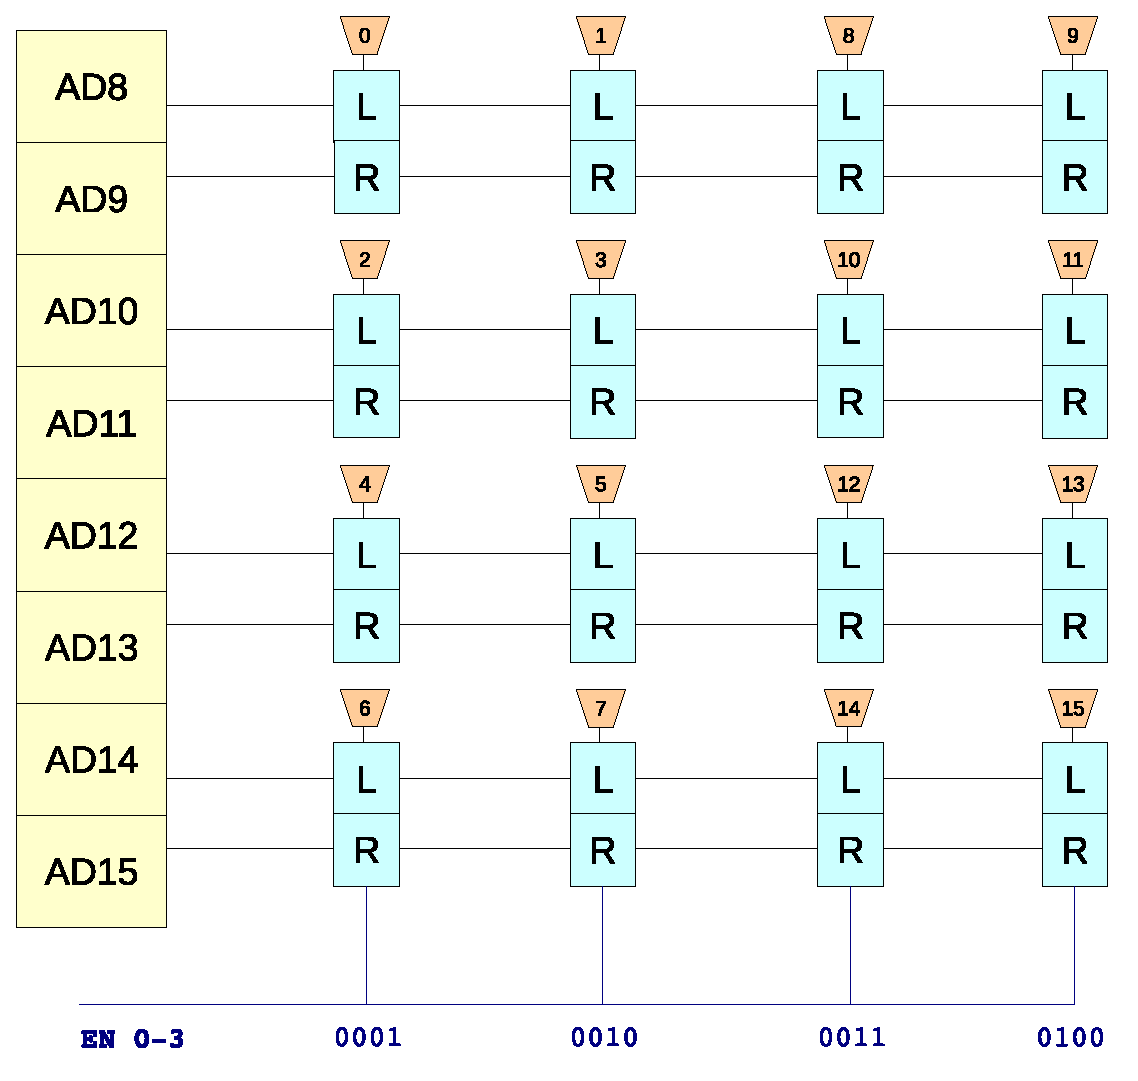
\includegraphics[width=11cm]{figure/AD24}
        \end{center}
        \figurecaption{Schema a blocchi della porta AD24}
         \label{fig:AD24}
\end{figure}
\end{center}
\`E possibile selezionare i feed su cui andare a leggere impostando sulla porta
DIO il valore di \texttt{EN 0-3}; come si vede in figura il valore \texttt{0001} di \texttt{EN 0-3} permette
di selezionare la prima colonna, il valore \texttt{0010} la seconda e cos\`i via per le altre due. La grandezza
da leggere invece dipende dal valore \texttt{AD 0-3} impostato nel DIO; questo permette di selezionare il valore di
$V_D$, $I_D$ o $V_G$ di uno dei cinque stadi degli LNA. La porta DIO \`e schematizzata in figura~\ref{fig:DIO}.
\begin{center}
\begin{figure}[!htbp]
        \begin{center}
        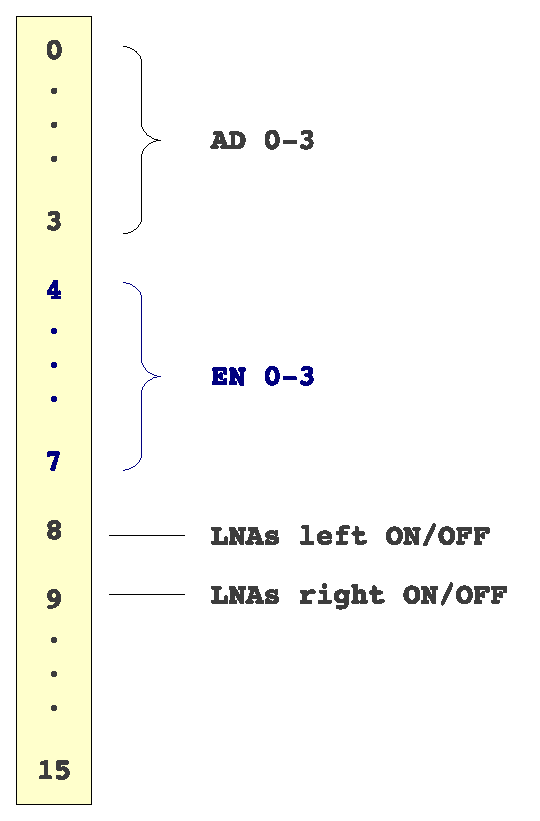
\includegraphics[width=5cm]{figure/DIO}
        \end{center}
        \figurecaption{Schema della porta DIO}
         \label{fig:DIO}
\end{figure}
\end{center}
Nella tabella~\ref{tab:AD03} sono indicati i valori di \texttt{AD 03} da impostare sulla porta DIO
per selezionare la grandezza da leggere.
\renewcommand\arraystretch{1.2}
\begin{table}[!htbp]
\begin{center}
\begin{tabular}{ c | c | p{4cm} }
\texttt{AD 0-3} & \textbf{Segnale} & \textbf{Stadio} \\
\hline 
\hline 
\texttt{0000} & $V_D$ & primo \\
\hline 
\texttt{0001} & $I_D$ & primo \\
\hline 
\texttt{0010} & $V_G$ & primo \\
\hline 
\texttt{0011} & $V_D$ & secondo \\
% \hline 
% \texttt{0100} & $I_D$ & secondo \\
% \hline 
% \texttt{0101} & $V_G$ & secondo \\
% \hline 
\dots & \dots & \dots \\
\hline
% \texttt{0110} & $V_D$ & terzo \\
% \hline 
% \texttt{0111} & $I_D$ & terzo \\
% \hline 
% \texttt{1000} & $V_G$ & terzo \\
% \hline 
% \texttt{1001} & $V_D$ & quarto \\
% \hline 
% \texttt{1010} & $I_D$ & quarto \\
% \hline 
% \texttt{1011} & $V_G$ & quarto \\
% \hline 
% \texttt{1100} & $V_D$ & quinto \\
% \hline 
% \texttt{1101} & $I_D$ & quinto \\
% \hline 
% \texttt{1110} & $V_G$ & quinto \\
% \hline 
\end{tabular}
\caption{Valori di \texttt{AD 0-3} per la selezione della grandezza da leggere}
\label{tab:AD03}
\end{center}
\end{table}

Supponiamo ad esempio di voler leggere gli 8 valori (4 feed, 2 canali per feed) di $V_G$ del terzo 
stadio dei feed 8, 10, 12 e 14. Il valore di \texttt{EN 0-3} sar\`a \texttt{0011} mentre il valore 
di \texttt{AD 0-3} sar\`a \texttt{1000}. Faremo allora due richieste: la prima (\texttt{SET\_DATA}\index{comando!set data}) 
ha lo scopo di configurare la porta DIO in modo da impostare i valori di 
\texttt{AD 0-3} e \texttt{EN 0-3}, mentre la seconda (\texttt{GET\_DATA}\index{comando!get data}) \`e la lettura della 
grandezza richiesta ($V_G$ del terzo stadio per i vari feed):
\begin{itemize}
\item \texttt{SET\_DATA}: avr\`a quattro \emph{parametri}\index{parametri}:
\begin{enumerate}
\item \textbf{data type}: unsigned da 8 bit
\item \textbf{port type}: DIO
\item \textbf{port number}: da 0 a 7 (8 bit, dall'indice 0 all'indice 7)
\item \textbf{value}: \texttt{10000011} (\texttt{AD 0-3} + \texttt{EN 0-3})
\end{enumerate}
\item \texttt{GET\_DATA}: avr\`a tre parametri\index{parametri}:
\begin{enumerate}
\item \textbf{data type}: 32 bit floating point
\item \textbf{port type}: AD24
\item \textbf{port number}: da 8 a 15
\end{enumerate}
\end{itemize}
Dopo aver dato il comando \texttt{SET\_DATA} \`e necessario attendere un \emph{tempo di guardia}\index{tempo di guardia} prima di
andare a leggere i valori con \texttt{GET\_DATA}, in modo da avere le uscite stabili; questo
tempo di guardia non deve essere inferiore ai $200$\,ms.

Il dato letto con il \texttt{GET\_DATA} \`e un 32 byte, che una volta scomposto in elementi da 4 byte ci fornisce
8 valori analogici di tensione, che andranno poi convertiti secondo opportune formule di trasformazione.


\subsection{Dewar Control Board}
Anche la scheda per il controllo del \emph{dewar}\index{dewar} ha una porta DIO ed una porta AD24, ma a differenza 
della scheda per il controllo degli LNA non \`e necessario scrivere sulla porta DIO prima di 
leggere dalla porta AD24, poich\`e non \`e possibile specificare quali grandezze leggere dalla porta
AD24; queste infatti non cambiano e sono le seguenti:
\begin{enumerate}
\item \texttt{AD08}: temperatura criogenica\index{temperatura!criogenica} numero 1;
\item \texttt{AD09}: temperatura criogenica numero 2;
\item \texttt{AD10}: pressione\index{pressione} all'interno del dewar;
\item \texttt{AD11}: temperatura criogenica numero 3;
\item \texttt{AD12}: temperatura criogenica numero 4;  
\item \texttt{AD13}: spare temperature\index{temperatura!spare};
\item \texttt{AD14}: vertex temperature{temperatura!vertex}\index{vertex};
\item \texttt{AD15}: spare temperature.
\end{enumerate}
I valori di tensione letti andranno poi convertiti tramite opportune formule in modo da ottenere i valori
nelle corrette unit\`a ingegneristiche (ad esempio in Kelvin o mbar).

Le porte ed i \emph{numeri di porta}\index{numeri di porta} descritti in questo documento sono relativi 
alle schede montate sul ricevitore
22 GHz multi-beam\index{ricevitore 22GHz} in funzione su SRT, ma le schede che verranno montate sui futuri ricevitori non dovrebbero
cambiare questa mappatura. I dettagli tecnici sulla scheda per il controllo degli LNA e su quella per
il controllo del dewar sono reperibili rispettivamente nei documenti~\cite{lna-controls}
e~\cite{dewar-controls}.

% Vediamo in questa sezione le principali operazioni che e
% del dewar. Indicare che i primi 16 bit possono essere scritti e letti, mentre i restanti 16 possono
% essere solo letti.
% \begin{enumerate}
% \item texttt{OUT\_00}: si pone il bit a 0 per selezionare l'oscillatore locale 1, mentre lo si
% pone ad 1 per selezionare l'oscillatore locale 2;
% \item texttt{OUT\_01}: libero
% \item texttt{OUT\_02}: libero
% \item texttt{OUT\_03}: 
% \item texttt{OUT\_04}:
% \item texttt{OUT\_05}:
% \item texttt{OUT\_06}:
% \item texttt{OUT\_07}:
% \item texttt{OUT\_08}:
% \item texttt{OUT\_09}:
% \item texttt{OUT\_10}:
% \item texttt{OUT\_11}: noise mark generator ON/OFF
% \item texttt{OUT\_12}: noise mark generator: external synchronous command enabled/disabled
% \item texttt{OUT\_13}: 
% \item texttt{OUT\_14}:
% \item texttt{OUT\_15}:
% \item texttt{IN\_00}: stato dell'oscillatore locale 1 (OL1). Quando il bit vale 1 allora OL1
% \`e selezionato;
% \item texttt{IN\_01}: stato dell'oscillatore locale 2 (OL2). Quando il bit vale 1 allora OL2
% \`e selezionato;
% \item texttt{IN\_02}: quando questo bit \`e a 1 OL2 \`e unlocked
% \item texttt{IN\_03}: remote/local
% \item texttt{IN\_04}: 
% \item texttt{IN\_05}: vacuum pump status
% \item texttt{IN\_06}: vacuum pump fault
% \item texttt{IN\_07}: vacuum valve status
% \item texttt{IN\_08}: 
% \item texttt{IN\_09}:
% \item texttt{IN\_10}:
% \item texttt{IN\_11}:
% \item texttt{IN\_12}:
% \item texttt{IN\_13}:
% \item texttt{IN\_14}:
% \item texttt{IN\_15}:
% \end{enumerate}


\section{Utilizzo della Libreria}
La \texttt{MicroControllerBoard} \`e una libreria thread-safe composta da~3 file: 
\emph{MicroControllerBoard.h} e \emph{MicroControllerBoard.cpp} nei quali viene rispettivamente
dichiarata e definita la classe \texttt{MicroControllerBoard}, ed il file \emph{MicroControllerBoardDef.h}
nel quale sono definiti tutti i parametri, come i \emph{tipi di dato}\index{tipo di dato}, le porte ed i numeri di porta.

Nel listato~\ref{lst:mcboard-getdata} \`e illustrato un breve esempio di utilizzo della
libreria, nel quale viene istanziato un oggetto MicroControllerBoard al fine di 
effettuare una richiesta \texttt{GET\_DATA}.
\lstset{language=C++}
\lstset{numbers=left,numberstyle={\scriptsize},stepnumber=1,firstnumber=1,numbersep=10pt}
\begin{lstlisting}[caption={[Esempio di utilizzo della libreria \texttt{MicroControllerBoard}]Esempio 
di utilizzo della libreria \texttt{MicroControllerBoard}},
label=lst:mcboard-getdata,mathescape]
#include "MicroControllerBoard.h"
#include <cstdlib>
using namespace IRA;

int main()
{
    // Definiamo i parametri IP e porta da passare al costruttore
    std::string IP("192.168.51.63"); // Indirizzo IP della scheda
    unsigned int port = 5002; // Numero di porta della connessione
    // Il vettore params conterra' i parametri del GET_DATA
    std::vector<BYTE> params;
    // Il data type e' un floating point a 32
    params.push_back(MCB_CMD_DATA_TYPE_F32);
    // La porta dalla quale leggere i dati e' la AD24
    params.push_back(MCB_PORT_TYPE_AD24); 
    // Vogliamo leggere un insieme di 8 dati floating point
    params.push_back(MCB_PORT_NUMBER_00_07);
    try {
        MicroControllerBoard mcb = MicroControllerBoard(IP, port);
        // Creiamo la connessione TCP/IP con la scheda
        mcb.openConnection();
        // Effettuiamo una richiesta GET_DATA
        mcb.send(MCB_CMD_GET_DATA, params);
        data = mcb.receive(); // Riceviamo i dati richiesti
        // Richiesta GET_DATA senza controllo checksum
        mcb.send(MCB_CMD_GET_DATA | MCB_CMD_TYPE_NOCHECKSUM, params);
        data = mcb.receive();
        mcb.closeConnection(); // Chiudiamo la connessione
    }
    catch(MicroControllerBoardEx& ex) {
        cout << ex.what() << endl;
        mcb.closeConnection();
        // ...
    }
    return 0;
}
\end{lstlisting}
\lstset{numbers=none}
Alle righe 11-17 viene creato il vettore di parametri che caratterizza la richiesta. I codici del
\textit{data type}, \textit{port type} e \textit{port number} sono definiti nel file
MicroControllerBoardDef.h, cos\`i come i codici dei comandi che vengono passati al metodo
\texttt{send} alle righe 23 e 26.

Quando nel metodo \texttt{send}\index{metodo!send} il codice di un comando viene messo in \texttt{or} con 
\texttt{MCB\_CMD\_TYPE\_NOCHECKSUM} (ad esempio, riga~26), significa che si sta effettuando
una comunicazione priva di controllo degli errori (nessun checksum).

Alle righe 24 e 27 viene invocato il metodo \texttt{receive}\index{metodo!receive}, il quale effettua tutti i 
possibili controlli sulla validit\`a della risposta:
\begin{itemize}
\item gli indirizzi del master\index{master} e dello slave\index{slave} della risposta devono coincidere con quelli della
richiesta;
\item il \emph{codice del comando}\index{codice del comando} deve essere valido;
\item risposta e richiesta devono avere lo stesso codice del comando;
\item l'identificativo (ID) della risposta deve essere lo stesso della richiesta;
\item il numero di parametri deve essere corretto;
\item il checksum\emph{checksum} (se richiesto) deve essere corretto.
\end{itemize}

\chapter{Receiver Control Library}

\section{Introduzione}
La \texttt{ReceiverControl} library definisce una interfaccia di alto livello
tramite la quale comunicare con il ricevitore. Poich\`e, come \`e stato detto, su ogni ricevitore
vengono installate due schede (una per il controllo del dewar\index{dewar} ed un'altra
per alimentare gli LNA\index{LNA} e leggerne i valori di $V_D$, $I_D$ e $V_G$), un oggetto \texttt{ReceiverControl}
istanzier\`a due \texttt{MicroControllerBoard}; questo come tutti gli altri dettagli di basso livello
sar\`a trasparente per l'utilizzatore della classe.

La libreria inoltre \`e \emph{thread-safe}\index{thread safe} in quanto per comunicare con 
le schede si appoggia alla \texttt{MicroControllerBoard}
(come detto nel capitolo precedente, la \texttt{MicroControllerBoard} \`e thread-safe).


\section{Interfaccia}
L'interfaccia della classe espone una serie di metodi che consentono di avere un completo controllo
del ricevitore. 

\subsection{Il Costruttore}
Nel listato~\ref{lst:costruttore}, mostrato di seguito, \`e riportata la dichiarazione del \emph{costruttore}\index{costruttore} 
della classe \texttt{ReceiverControl}.
\lstset{language=C++}
\lstset{numbers=left,numberstyle={\scriptsize},stepnumber=1,firstnumber=1,numbersep=10pt}
\begin{lstlisting}[caption={[Dichiarazione del costruttore di \texttt{ReceiverControl}]
Dichiarazione del costruttore della classe \texttt{ReceiverControl}},
label=lst:costruttore,mathescape]
ReceiverControl(
        const std::string dewar_ip,
        const unsigned short dewar_port, 
        const std::string lna_ip, 
        const unsigned short lna_port, 
        const unsigned short number_of_feeds=1,
        const BYTE dewar_madd=0x7C, // Dewar board master address
        const BYTE dewar_sadd=0x7D, // Dewar board slave address
        const BYTE lna_madd=0x7C,   // LNA board master address
        const BYTE lna_sadd=0x7D,   // LNA board slave address
        bool reliable_comm=true,
        const unsigned int guard_time=250000  // 0.25 seconds
) throw (ReceiverControlEx);
\end{lstlisting}
\lstset{numbers=none}
I parametri hanno il seguente significato:
\begin{itemize}
\item \texttt{dewar\_ip}\index{parametri costruttore!dewar IP}: l'indirizzo IP della scheda per il controllo del dewar;
\item \texttt{dewar\_port}\index{parametri costruttore!dewar port}: la porta utilizzata nella 
connessione verso la scheda per il controllo del dewar;
\item \texttt{lna\_ip}\index{parametri costruttore!LNA IP}: l'indirizzo IP della scheda per il controllo degli LNA;
\item \texttt{lna\_port}\index{parametri costruttore!LNA port}: la porta utilizzata nella 
connessione verso la scheda per il controllo degli LNA;
\item \texttt{number\_of\_feeds}\index{parametri costruttore!numero di feeds}: numero di feed del ricevitore (1 di default);
\item \texttt{dewar\_maddr}\index{parametri costruttore!dewar master address}: l'indirizzo del master della
scheda del dewar (il valore di default \`e 0x7D);
\item \texttt{dewar\_saddr}\index{parametri costruttore!dewar slave address} l'indirizzo dello slave della 
scheda del dewar (il valore di default \`e 0x7F)
\item \texttt{lna\_maddr}\index{parametri costruttore!LNA master address}: l'indirizzo del master della 
scheda degli LNA (il valore di default \`e 0x7D);
\item \texttt{lna\_saddr}\index{parametri costruttore!LNA slave address}: l'indirizzo dello slave della 
scheda degli LNA (il valore di default \`e 0x7F)
\item \texttt{reliable\_comm}\index{parametri costruttore!reliable communication}: 
quando vale  \texttt{true} allora la comunicazione con le schede avviene
con controllo degli errori (checksum)\index{checksum}. Di default \`e \texttt{true};
\item \texttt{guard\_time}\index{parametri costruttore!tempo di guardia}\index{tempo di guardia}: 
quando viene fatta una richiesta di lettura dei dati alla scheda degli LNA,
dobbiamo aspettare un certo lasso di tempo prima di leggere il dato richiesto, in modo tale che le
uscite si stabilizzino. Questo tempo non deve essere inferiore ai 200ms ed \`e impostabile tramite questo
parametro.
\end{itemize}
    
\subsection{Il metodo \texttt{fetValues}}
Il metodo \texttt{fetValues}\index{metodo!fetValues} restituisce la struttura \texttt{FetValues} di un LNA
per un dato stadio e per un dato feed. La struttura \`e definita di seguito:
\lstset{language=C++}
\lstset{numbers=left,numberstyle={\scriptsize},stepnumber=1,firstnumber=1,numbersep=10pt}
\begin{lstlisting}[mathescape]
struct FetValues {
    double VDL; // Drain Voltage, left channel  [V]
    double IDL; // Drain Current, left channel  [mA]
    double VGL; // Gate Voltage, left channel   [V]
    double VDR; // Drain Voltage, right channel [V]
    double IDR; // Drain Current, right channel [mA]
    double VGR; // Gate Voltage, right channel  [V]
};
\end{lstlisting}
\lstset{numbers=none}
Per poter restiture la struttura~\texttt{FetValues} dobbiamo quindi passare al metodo \texttt{fetValues} i seguenti
parametri: 
\begin{itemize}
\item il codice identificativo del feed;
\item il numero dello stadio;
\item un puntatore alla funzione di conversione che, a partire dal valore
in tensione letto, lo converte in un valore di corrente (IDL e IDR);
\item un puntatore alla funzione 
che converte il valore letto nel corretto valore di tensione (VDL, VGL, VDR, VGR).
\end{itemize}
\lstset{language=C++}
\lstset{numbers=left,numberstyle={\scriptsize},stepnumber=1,firstnumber=1,numbersep=10pt}
\begin{lstlisting}[caption={Dichiarazione del metodo \texttt{fetValues}},
label=lst:fetValues,mathescape]
/** return the FetValues (VDL, IDL, VGR, VDR, IDR and VGR) 
 *  of the LNA of the feed `feed_number` and stage `stage_number`. 
 *  The letter L means that the value is referred to the left 
 *  channel, the R if for the right one.
 *  @param feed_number the ID code of the feed (from 0 to 15)
 *  @param stage_number the stage number (from 1 to 5)
 *  @param currentConverter pointer to the function that performs 
 *  the conversion from voltage to mA; default value is NULL, 
 *  and in this case the value of ID is the voltage value (the 
 *  value before conversion).
 *  @param voltageConverter pointer to the function that performs 
 *  the conversion from voltage to voltage; default value is NULL, 
 *  and in this case the values of VD and VG are the voltage values 
 *  before the conversion.
 *  @return the low cryogenic temperature in Kelvin if 
 *  converter != NULL, the value in voltage (before conversion) 
 *  otherwise.
 *  @return the FetValues, a struct of three double members: 
 *  VD [V], ID [mA] and VG [V] after the conversion if the 
 *  function pointers are not NULL, the values before conversion 
 *  (voltage) if the pointers are NULL.
 *  @throw ReceiverControlEx
 */
FetValues fetValues(
        unsigned short feed_number, 
        unsigned short stage_number,
        double (*currentConverter)(double voltage) = NULL,
        double (*voltageConverter)(double voltage) = NULL
) throw (ReceiverControlEx);
\end{lstlisting}
\lstset{numbers=none}


\subsection{Il metodo \texttt{stageValues}}
Il metodo \texttt{stageValues}\index{metodo!stageValues} prende come parametri: un elemento \texttt{FetValue} (ovvero
\texttt{DRAIN\_VOLTAGE}\index{drain voltage}, \texttt{DRAIN\_CURRENT}\index{drain current} o 
\texttt{GATE\_VOLTAGE}\index{gate voltage}), lo stadio
di amplificazione (un intero compreso tra~1 e~5), un puntatore ad una funzione che effettua
la conversione del valore letto nel corrispondente valore di tensione o corrente, a seconda
della grandezza richiesta (primo parametro).

Il tipo restituito \`e uno \texttt{StageValues}:
\lstset{language=C++}
\lstset{numbers=left,numberstyle={\scriptsize},stepnumber=1,firstnumber=1,numbersep=10pt}
\begin{lstlisting}[mathescape]
/**
 * The left_channel member stores all the left channel values of a
 * specific fet quantity (VD, ID or VG), and the right one stores 
 * the values for the right channel.
 */
struct StageValues {
    std::vector<double> left_channel;
    std::vector<double> right_channel;
};
\end{lstlisting}
\lstset{numbers=none}
Il membro \texttt{left\_channel} \`e un vettore che ha come elementi i valori della grandezza richiesta (il
primo parametro del metodo), per lo stadio di amplificazione richiesto, ordinati per feed;
il primo elemento del vettore \`e quindi riferito al primo feed, il secondo elemento al 
secondo feed e cos\`i via. Stessa cosa per quanto riguarda il vettore \texttt{right\_channel}.
Per poter recuperare questi valori, sulla base di quanto descritto in~\ref{sec:lna-section}, dobbiamo fare un 
numero di richeste \texttt{GET\_DATA} che dipende solo dal numero di feed\footnote{Nel caso del 
ricevitore 22GHz multi-beem ad esempio, avendo questo~7 feed dovremo fare~2 richieste \texttt{GET\_DATA},
poich\`e sono 2 le colonne da leggere, come si evince dallo schema di figura~\ref{fig:AD24}.}.
\lstset{language=C++}
\lstset{numbers=left,numberstyle={\scriptsize},stepnumber=1,firstnumber=1,numbersep=10pt}
\begin{lstlisting}[caption={Dichiarazione del metodo \texttt{stageValues}},
label=lst:stageValues,mathescape]
/** Return for each feed and channel the fet quantity value of 
 *  a given stage. For instance, if you want to get the VD values 
 *  of all the feeds related to the amplifier stage N, you must 
 *  call the method like so: stageValues(DRAIN_VOLTAGE, N).
 *
 *  @param quantity a FetValue: DRAIN_VOLTAGE, DRAIN_CURRENT 
 *  or GATE_CURRENT 
 *  @param stage_number the stage number (from 1 to 5)
 *  @param converter pointer to the function that performs the 
 *  conversion from voltage to the right unit or just with a 
 *  scale factor; default value is NULL, and in this case the 
 *  value returned is without conversion.
 *  @return the StageValues for a given fet ``quantity`` and 
 *  ``stage_number``. The StageValues is a struct of two 
 *  members std::vector<double>, one member for the left 
 *  channel and one for the right one. That members contain 
 *  the related quantities of all the feeds; that means each
 *  item of the std::vector<double> is the quantity value of 
 *  a feed, for the stage requested.
 *  @throw ReceiverControlEx
 */
 StageValues stageValues(
         FetValue quantity, 
         unsigned short stage_number, 
         double (*converter)(double voltage)=NULL
) throw (ReceiverControlEx);
\end{lstlisting}
\lstset{numbers=none}


\subsection{Il metodo \texttt{turnLeftLNAsOn}}
Il metodo \texttt{turnLeftLNAsOn}\index{metodo!turnLeftLNAsOn} accende tutti gli LNA dei canali left.
\lstset{language=C++}
\lstset{numbers=left,numberstyle={\scriptsize},stepnumber=1,firstnumber=1,numbersep=10pt}
\begin{lstlisting}[caption={Dichiarazione del metodo \texttt{turnLeftLNAsOn}},
label=lst:turnLeftLNAsOn,mathescape]
/** Turn the LNAs of the left channels ON
 *  @param data_type the type of the data; the default is 1 bit
 *  @param port_type the port type; the default is the Digital IO
 *  @param port_number the port number; the default is 08
 *  @param value the value to set; the default value is 0x00
 *  @throw ReceiverControlEx
 */
void turnLeftLNAsOn(
        const BYTE data_type=MCB_CMD_DATA_TYPE_B01,
        const BYTE port_type=MCB_PORT_TYPE_DIO,
        const BYTE port_number=MCB_PORT_NUMBER_08,
        const BYTE value=0x00
) throw (ReceiverControlEx);
\end{lstlisting}
\lstset{numbers=none}


\subsection{Il metodo \texttt{turnLeftLNAsOff}}
Il metodo \texttt{turnLeftLNAsOff}\index{metodo!turnLeftLNAsOff} spegne tutti gli LNA dei canali left.
\lstset{language=C++}
\lstset{numbers=left,numberstyle={\scriptsize},stepnumber=1,firstnumber=1,numbersep=10pt}
\begin{lstlisting}[caption={Dichiarazione del metodo \texttt{turnLeftLNAsOff}},
label=lst:turnLeftLNAsOff,mathescape]
/** Turn the LNAs of the left channels OFF
 *  @param data_type the type of the data; the default is 1 bit
 *  @param port_type the port type; the default is the Digital IO
 *  @param port_number the port number; the default port number is 08
 *  @param value the value to set; the default value is 0x01
 *  @throw ReceiverControlEx
 */
void turnLeftLNAsOff(
        const BYTE data_type=MCB_CMD_DATA_TYPE_B01,
        const BYTE port_type=MCB_PORT_TYPE_DIO,
        const BYTE port_number=MCB_PORT_NUMBER_08,
        const BYTE value=0x01
) throw (ReceiverControlEx);
\end{lstlisting}
\lstset{numbers=none}


\subsection{Il metodo \texttt{turnRightLNAsOn}}
Il metodo \texttt{turnRightLNAsOn}\index{metodo!turnRightLNAsOn} accende tutti gli LNA dei canali right.
\lstset{language=C++}
\lstset{numbers=left,numberstyle={\scriptsize},stepnumber=1,firstnumber=1,numbersep=10pt}
\begin{lstlisting}[caption={Dichiarazione del metodo \texttt{turnRightLNAsOn}},
label=lst:turnRightLNAsOn,mathescape]
/** Turn the LNAs of the right channels ON
 *  @param data_type the type of the data; the default is 1 bit
 *  @param port_type the port type; the default is the Digital IO
 *  @param port_number the port number; the default is 09
 *  @param value the value to set; the default value is 0x00
 *  @throw ReceiverControlEx
 */
void turnRightLNAsOn(
        const BYTE data_type=MCB_CMD_DATA_TYPE_B01,
        const BYTE port_type=MCB_PORT_TYPE_DIO,
        const BYTE port_number=MCB_PORT_NUMBER_09,
        const BYTE value=0x00 
) throw (ReceiverControlEx);
\end{lstlisting}
\lstset{numbers=none}


\subsection{Il metodo \texttt{turnRightLNAsOff}}
Il metodo \texttt{turnRightLNAsOff}\index{metodo!turnRightLNAsOff} spegne tutti gli LNA dei canali right.
\lstset{language=C++}
\lstset{numbers=left,numberstyle={\scriptsize},stepnumber=1,firstnumber=1,numbersep=10pt}
\begin{lstlisting}[caption={Dichiarazione del metodo \texttt{turnRightLNAsOff}},
label=lst:turnRightLNAsOff,mathescape]
/** Turn the LNAs of the right channels OFF
 *  @param data_type the type of the data; the default is 1 bit
 *  @param port_type the port type; the default is the Digital IO
 *  @param port_number the port number; the default is 09
 *  @param value the value to set; the default value is 0x01
 *  @throw ReceiverControlEx
 */
void turnRightLNAsOff(
        const BYTE data_type=MCB_CMD_DATA_TYPE_B01,
        const BYTE port_type=MCB_PORT_TYPE_DIO,
        const BYTE port_number=MCB_PORT_NUMBER_09,
        const BYTE value=0x01
) throw (ReceiverControlEx);
\end{lstlisting}
\lstset{numbers=none}

\subsection{Il metodo \texttt{setCalibrationOn}}
Il metodo \texttt{setCalibrationOn}\index{metodo!setCalibrationOn} avvia la calibrazione del ricevitore mediante 
una marca di rumore.
\lstset{language=C++}
\lstset{numbers=left,numberstyle={\scriptsize},stepnumber=1,firstnumber=1,numbersep=10pt}
\begin{lstlisting}[caption={Dichiarazione del metodo \texttt{setCalibrationOn}},
label=lst:setCalibrationOn,mathescape]
/** Set the noise mark generator to ON 
 *  @param data_type the type of the data; the default is 1 bit
 *  @param port_type the port type; the default is the Digital IO
 *  @param port_number the port number; the default is 11
 *  @param value the value to set; the default value is 0x01
 *  @throw ReceiverControlEx
 */
void setCalibrationOn(
        const BYTE data_type=MCB_CMD_DATA_TYPE_B01, 
        const BYTE port_type=MCB_PORT_TYPE_DIO, 
        const BYTE port_number=MCB_PORT_NUMBER_11, 
        const BYTE value=0x01
) throw (ReceiverControlEx);
\end{lstlisting}
\lstset{numbers=none}


\subsection{Il metodo \texttt{setCalibrationOff}}
Il metodo \texttt{setCalibrationOff}\index{metodo!setCalibrationOff} ferma la calibrazione del ricevitore.
\lstset{language=C++}
\lstset{numbers=left,numberstyle={\scriptsize},stepnumber=1,firstnumber=1,numbersep=10pt}
\begin{lstlisting}[caption={Dichiarazione del metodo \texttt{setCalibrationOff}},
label=lst:setCalibrationOff,mathescape]
/** Set the noise mark generator to OFF
 *  @param data_type the type of the data; the default is 1 bit
 *  @param port_type the port type; the default is the Digital IO
 *  @param port_number the port number; the default is 11
 *  @param value the value to set; the default value is 0x00
 *  @throw ReceiverControlEx
 */
void setCalibrationOff(
        const BYTE data_type=MCB_CMD_DATA_TYPE_B01, 
        const BYTE port_type=MCB_PORT_TYPE_DIO, 
        const BYTE port_number=MCB_PORT_NUMBER_11, 
        const BYTE value=0x00
) throw (ReceiverControlEx);
\end{lstlisting}
\lstset{numbers=none}


\subsection{Il metodo \texttt{isCalibrationOn}}
Il metodo \texttt{isCalibrationOn}\index{metodo!isCalibrationOn} restituisce \texttt{true} se la calibrazione del 
ricevitore \`e attiva.
\lstset{language=C++}
\lstset{numbers=left,numberstyle={\scriptsize},stepnumber=1,firstnumber=1,numbersep=10pt}
\begin{lstlisting}[caption={Dichiarazione del metodo \texttt{isCalibrationOn}},
label=lst:isCalibrationOn,mathescape]
/** Is the noise mark generator set to ON?
 *  @param data_type the type of the data; the default is 1 bit
 *  @param port_type the port type; the default is the Digital IO
 *  @param port_number the port number; the default is 11
 *  @return true if the noise mark generator is set to ON
 *  @throw ReceiverControlEx
 */
bool isCalibrationOn(
        const BYTE data_type=MCB_CMD_DATA_TYPE_B01, 
        const BYTE port_type=MCB_PORT_TYPE_DIO, 
        const BYTE port_number=MCB_PORT_NUMBER_11
) throw (ReceiverControlEx);
\end{lstlisting}
\lstset{numbers=none}


\subsection{Il metodo \texttt{setExtCalibrationOn}}
Il metodo \texttt{setExtCalibrationOn}\index{metodo!setExtCalibrationOn} abilita il comando esterno per la calibrazione.
ricevitore \`e attiva.
\lstset{language=C++}
\lstset{numbers=left,numberstyle={\scriptsize},stepnumber=1,firstnumber=1,numbersep=10pt}
\begin{lstlisting}[caption={Dichiarazione del metodo \texttt{setExtCalibrationOn}},
label=lst:setExtCalibrationOn,mathescape]
/** Enable the external noise mark generator synchronous command
 *  @param data_type the type of the data; the default is 1 bit
 *  @param port_type the port type; the default is the Digital IO
 *  @param port_number the port number; the default is 12
 *  @param value the value to set; the default value is 0x01
 *  @throw ReceiverControlEx
 */
void setExtCalibrationOn(
        const BYTE data_type=MCB_CMD_DATA_TYPE_B01, 
        const BYTE port_type=MCB_PORT_TYPE_DIO, 
        const BYTE port_number=MCB_PORT_NUMBER_12, 
        const BYTE value=0x01
) throw (ReceiverControlEx);
\end{lstlisting}
\lstset{numbers=none}


\subsection{Il metodo \texttt{setExtCalibrationOff}}
Il metodo \texttt{setExtCalibrationOff}\index{metodo!setExtCalibrationOff} disabilita il comando esterno per fermare la calibrazione.
\lstset{language=C++}
\lstset{numbers=left,numberstyle={\scriptsize},stepnumber=1,firstnumber=1,numbersep=10pt}
\begin{lstlisting}[caption={Dichiarazione del metodo \texttt{setExtCalibrationOff}},
label=lst:setExtCalibrationOff,mathescape]
/** Disable the external noise mark generator synchronous command
 *  @param data_type the type of the data; the default is 1 bit
 *  @param port_type the port type; the default is the Digital IO
 *  @param port_number the port number; the default is 12
 *  @param value the value to set; the default value is 0x00
 *  @throw ReceiverControlEx
 */
void setExtCalibrationOff(
        const BYTE data_type=MCB_CMD_DATA_TYPE_B01, 
        const BYTE port_type=MCB_PORT_TYPE_DIO, 
        const BYTE port_number=MCB_PORT_NUMBER_12, 
        const BYTE value=0x00
) throw (ReceiverControlEx);
\end{lstlisting}
\lstset{numbers=none}


\subsection{Il metodo \texttt{isExtCalibrationOn}}
Il metodo \texttt{isExtCalibrationOn}\index{metodo!isExtCalibrationOn} restituisce \texttt{true} se il comando esterno 
per avviare la calibrazione \`e abilitato.
\lstset{language=C++}
\lstset{numbers=left,numberstyle={\scriptsize},stepnumber=1,firstnumber=1,numbersep=10pt}
\begin{lstlisting}[caption={Dichiarazione del metodo \texttt{isExtCalibrationOn}},
label=lst:isExtCalibrationOn,mathescape]
/** Is the external noise mark generator command enabled?
 *  @param data_type the type of the data; the default is 1 bit
 *  @param port_type the port type; the default is the Digital IO
 *  @param port_number the port number; the default is 12
 *  @return true if the external noise mark generator command 
 *  is enabled
 *  @throw ReceiverControlEx
 */
bool isExtCalibrationOn(
        const BYTE data_type=MCB_CMD_DATA_TYPE_B01, 
        const BYTE port_type=MCB_PORT_TYPE_DIO, 
        const BYTE port_number=MCB_PORT_NUMBER_12
) throw (ReceiverControlEx);
\end{lstlisting}
\lstset{numbers=none}


\subsection{Il metodo \texttt{setReliableCommOn}}
Il metodo \texttt{setReliableCommOn}\index{metodo!setReliableCommOn} attiva la comunicazione con 
controllo degli errori (checksum)\index{checksum}.
\lstset{language=C++}
\lstset{numbers=left,numberstyle={\scriptsize},stepnumber=1,firstnumber=1,numbersep=10pt}
\begin{lstlisting}[caption={Dichiarazione del metodo \texttt{setReliableCommOn}},
label=lst:setReliableCommOn,mathescape]
/** Set the reliable communication to/from the board to ON */
void setReliableCommOn() { m_reliable_comm = true; }
\end{lstlisting}
\lstset{numbers=none}


\subsection{Il metodo \texttt{setReliableCommOff}}
Il metodo \texttt{setReliableCommOff}\index{metodo!setReliableCommOff} disattiva la 
comunicazione con controllo degli errori (nessun checksum)\index{checksum}.
\lstset{language=C++}
\lstset{numbers=left,numberstyle={\scriptsize},stepnumber=1,firstnumber=1,numbersep=10pt}
\begin{lstlisting}[caption={Dichiarazione del metodo \texttt{setReliableCommOff}},
label=lst:setReliableCommOff,mathescape]
/** Set the reliable communication to/from the board to OFF */
void setReliableCommOff() { m_reliable_comm = false; }
\end{lstlisting}
\lstset{numbers=none}


\subsection{Il metodo \texttt{isReliableCommOn}\index{metodo!isReliableCommOn}}
\lstset{language=C++}
\lstset{numbers=left,numberstyle={\scriptsize},stepnumber=1,firstnumber=1,numbersep=10pt}
\begin{lstlisting}[caption={Dichiarazione del metodo \texttt{isReliableCommOn}},
label=lst:isReliableCommOn,mathescape]
/** return true if the communication to the board is 
 *  set to be reliable 
 */
bool isReliableCommOn() { return m_reliable_comm; }
\end{lstlisting}
\lstset{numbers=none}


\subsection{Il metodo \texttt{vacuum}}
Il metodo \texttt{vacuum}\index{vacuum}\index{metodo!vacuum} restituisce la pressione\index{pressione} 
(in $mbar$) all'interno del dewar.
\lstset{language=C++}
\lstset{numbers=left,numberstyle={\scriptsize},stepnumber=1,firstnumber=1,numbersep=10pt}
\begin{lstlisting}[caption={Dichiarazione del metodo \texttt{vacuum}},
label=lst:vacuum,mathescape]
/** Return the vacuum value inside the dewar in mbar
 *
 *  @param converter pointer to the function that performs 
 *  the conversion from voltage to vacumm unit [mbar]; 
 *  default value is NULL, and in this case the value
 *  returned by vacuum is the voltage value (the value 
 *  before conversion).
 *  @param data_type the type of the data; the default 
 *  type is a 32 bit floating point
 *  @param port_type the port type; the default is the AD24
 *  @param port_number the port number; the default value 
 *  is a range of port numbers from 8 to 15.
 *  @param raw_index the index that allows to get the vacuum 
 *  value from the port_number range.
 *  The default value is 2.
 *  @return the vacuum inside the dewar in mbar if 
 *  converter != NULL, the value before conversion otherwise.
 *  @throw ReceiverControlEx
 */
double vacuum(
        double (*converter)(double voltage)=NULL,
        const BYTE data_type=MCB_CMD_DATA_TYPE_F32,     
        const BYTE port_type=MCB_PORT_TYPE_AD24,       
        const BYTE port_number=MCB_PORT_NUMBER_00_07,  
        const size_t raw_index=2                      
) throw (ReceiverControlEx);
\end{lstlisting}
\lstset{numbers=none}


\subsection{Il metodo \texttt{vertexTemperature}\index{metodo!vacuum}\index{temperatura!vertex}\index{vertex}}
\lstset{language=C++}
\lstset{numbers=left,numberstyle={\scriptsize},stepnumber=1,firstnumber=1,numbersep=10pt}
\begin{lstlisting}[caption={Dichiarazione del metodo \texttt{vertexTemperature}},
label=lst:vertexTemperature,mathescape]
/** Return the vertex temperature in K
 *  @param converter pointer to the function that 
 *  performs the conversion from voltage to Kelvin; 
 *  default value is NULL, and in this case the value
 *  returned by vertexTemperature is the voltage value 
 *  (the value before conversion).
 *  @param data_type the type of the data; the default 
 *  type is a 32 bit floating point
 *  @param port_type the port type; the default is the AD24
 *  @param port_number the port number; the default value 
 *  is a range of port numbers from 8 to 15.
 *  @param raw_index the index that allows to get the 
 *  vertex temperature value from the port_number range. 
 *  The default value is 6.
 *  @return the vertex temperature in Kelvin if 
 *  converter != NULL, the value before conversion otherwise.
 *  @throw ReceiverControlEx
 */
double vertexTemperature(
        double (*converter)(double voltage)=NULL,
        const BYTE data_type=MCB_CMD_DATA_TYPE_F32,     
        const BYTE port_type=MCB_PORT_TYPE_AD24,       
        const BYTE port_number=MCB_PORT_NUMBER_00_07,  
        const size_t raw_index=6                      
) throw (ReceiverControlEx);
\end{lstlisting}
\lstset{numbers=none}


\subsection{Il metodo \texttt{cryoTemperature}\index{metodo!cryoTemperature}}
\lstset{language=C++}
\lstset{numbers=left,numberstyle={\scriptsize},stepnumber=1,firstnumber=1,numbersep=10pt}
\begin{lstlisting}[caption={Dichiarazione del metodo \texttt{cryoTemperature}},
label=lst:cryoTemperature,mathescape]
/** Return the cryogenic temperature
 *  @param temperature_id the id code of the 
 *  temperature (1, 2, 3 or 4)
 *  @param converter pointer to the function 
 *  that performs the conversion from
 *  voltage to Kelvin; default value is NULL,
 *  and in this case the value returned by 
 *  cryoTemperature is the voltage value (the 
 *  value before conversion).
 *  @param data_type the type of the data; the 
 *  default type is a 32 bit floating point
 *  @param port_type the port type; the default is the AD24
 *  @param port_number the port number; the default value 
 *  is a range of port numbers from 8 to 15.
 *  @return the cryogenic temperature in Kelvin if 
 *  converter != NULL, the value in voltage (before 
 *  conversion) otherwise.
 *  @throw ReceiverControlEx
 */
double cryoTemperature(
        const short temperature_id,
        double (*converter)(double voltage)=NULL,
        const BYTE data_type=MCB_CMD_DATA_TYPE_F32,
        const BYTE port_type=MCB_PORT_TYPE_AD24,  
        const BYTE port_number=MCB_PORT_NUMBER_00_07
) throw (ReceiverControlEx);
\end{lstlisting}
\lstset{numbers=none}


\subsection{Il metodo \texttt{setCoolHeadOn}\index{metodo!setCoolHeadOn}\index{cool head}}
\lstset{language=C++}
\lstset{numbers=left,numberstyle={\scriptsize},stepnumber=1,firstnumber=1,numbersep=10pt}
\begin{lstlisting}[caption={Dichiarazione del metodo \texttt{setCoolHeadOn}},
label=lst:setCoolHeadOn,mathescape]
/** Set to ON the cool head 
 *  @param data_type the type of the data; the default is 1 bit
 *  @param port_type the port type; the default is the Digital IO
 *  @param port_number the port number; the default is 08
 *  @param value the value to set; the default value is 0x01
 *  @throw ReceiverControlEx
 */
void setCoolHeadOn(
        const BYTE data_type=MCB_CMD_DATA_TYPE_B01,
        const BYTE port_type=MCB_PORT_TYPE_DIO,   
        const BYTE port_number=MCB_PORT_NUMBER_08,
        const BYTE value=0x01
) throw (ReceiverControlEx);
\end{lstlisting}
\lstset{numbers=none}


\subsection{Il metodo \texttt{setCoolHeadOff}\index{metodo!setCoolHeadOff}}
\lstset{language=C++}
\lstset{numbers=left,numberstyle={\scriptsize},stepnumber=1,firstnumber=1,numbersep=10pt}
\begin{lstlisting}[caption={Dichiarazione del metodo \texttt{setCoolHeadOff}},
label=lst:setCoolHeadOff,mathescape]
/** Set to OFF the cool head 
 *  @param data_type the type of the data; the default is 1 bit
 *  @param port_type the port type; the default is the Digital IO
 *  @param port_number the port number; the default is 08
 *  @param value the value to set; the default value is 0x00
 *  @throw ReceiverControlEx
 */
void setCoolHeadOff(
        const BYTE data_type=MCB_CMD_DATA_TYPE_B01,
        const BYTE port_type=MCB_PORT_TYPE_DIO,   
        const BYTE port_number=MCB_PORT_NUMBER_08,
        const BYTE value=0x00
) throw (ReceiverControlEx);
\end{lstlisting}
\lstset{numbers=none}


\subsection{Il metodo \texttt{isCoolHeadOn}\index{metodo!isCoolHeadOn}}
\lstset{language=C++}
\lstset{numbers=left,numberstyle={\scriptsize},stepnumber=1,firstnumber=1,numbersep=10pt}
\begin{lstlisting}[caption={Dichiarazione del metodo \texttt{isCoolHeadOn}},
label=lst:isCoolHeadOn,mathescape]
/** Is the cool head ON?
 *  @param data_type the type of the data; the default is 1 bit
 *  @param port_type the port type; the default is the Digital IO
 *  @param port_number the port number; the default number is 08
 *  @return true if the cool head is ON
 *  @throw ReceiverControlEx
 */
bool isCoolHeadOn(
        const BYTE data_type=MCB_CMD_DATA_TYPE_B01,
        const BYTE port_type=MCB_PORT_TYPE_DIO,   
        const BYTE port_number=MCB_PORT_NUMBER_08
) throw (ReceiverControlEx);
\end{lstlisting}
\lstset{numbers=none}


\subsection{Il metodo \texttt{setVacuumSensorOn}\index{metodo!setVacuumSensorOn}}
Il metodo \texttt{setVacuumSensorOn} attiva il sensore di pressione\index{pressione}.
\lstset{language=C++}
\lstset{numbers=left,numberstyle={\scriptsize},stepnumber=1,firstnumber=1,numbersep=10pt}
\begin{lstlisting}[caption={Dichiarazione del metodo \texttt{setVacuumSensorOn}},
label=lst:setVacuumSensorOn,mathescape]
/** Set to ON the vacuum sensor
 *  @param data_type the type of the data; the default is 1 bit
 *  @param port_type the port type; the default is the Digital IO
 *  @param port_number the port number; the default is 04
 *  @param value the value to set; the default value is 0x01
 *  @throw ReceiverControlEx
 */
void setVacuumSensorOn(
        const BYTE data_type=MCB_CMD_DATA_TYPE_B01,
        const BYTE port_type=MCB_PORT_TYPE_DIO,
        const BYTE port_number=MCB_PORT_NUMBER_04,
        const BYTE value=0x01
) throw (ReceiverControlEx);
\end{lstlisting}
\lstset{numbers=none}


\subsection{Il metodo \texttt{setVacuumSensorOff}\index{metodo!setVacuumSensorOff}}
Il metodo \texttt{setVacuumSensorOff} disattiva il sensore di pressione\index{pressione}.
\lstset{language=C++}
\lstset{numbers=left,numberstyle={\scriptsize},stepnumber=1,firstnumber=1,numbersep=10pt}
\begin{lstlisting}[caption={Dichiarazione del metodo \texttt{setVacuumSensorOff}},
label=lst:setVacuumSensorOff,mathescape]
/** Set to OFF the vacuum sensor
 *  @param data_type the type of the data; the default is 1 bit
 *  @param port_type the port type; the default is the Digital IO
 *  @param port_number the port number; the default is 04
 *  @param value the value to set; the default value is 0x00
 *  @throw ReceiverControlEx
 */
void setVacuumSensorOff(
        const BYTE data_type=MCB_CMD_DATA_TYPE_B01,
        const BYTE port_type=MCB_PORT_TYPE_DIO,
        const BYTE port_number=MCB_PORT_NUMBER_04,
        const BYTE value=0x00
) throw (ReceiverControlEx);
\end{lstlisting}
\lstset{numbers=none}


\subsection{Il metodo \texttt{isVacuumSensorOn}}
Il metodo \texttt{isVacuumSensorOn}\index{metodo!isVacuumSensorOn} restituisce true se il sensore di pressione\index{pressione}
\`e attivo.
\lstset{language=C++}
\lstset{numbers=left,numberstyle={\scriptsize},stepnumber=1,firstnumber=1,numbersep=10pt}
\begin{lstlisting}[caption={Dichiarazione del metodo \texttt{isVacuumSensorOn}},
label=lst:isVacuumSensorOn,mathescape]
/** Is the vacuum sensor ON?
 *  @param data_type the type of the data; the default is 1 bit
 *  @param port_type the port type; the default is the Digital IO
 *  @param port_number the port number; the default is 04
 *  @return true if the vacuum sensor is ON 
 *  @throw ReceiverControlEx
 */
bool isVacuumSensorOn(
        const BYTE data_type=MCB_CMD_DATA_TYPE_B01,
        const BYTE port_type=MCB_PORT_TYPE_DIO,
        const BYTE port_number=MCB_PORT_NUMBER_04
) throw (ReceiverControlEx);
\end{lstlisting}
\lstset{numbers=none}


\subsection{Il metodo \texttt{setVacuumPumpOn}}
Il metodo \texttt{setVacuumPumpOn}\index{metodo!setVacuumPumpOn} attiva la \emph{pompa a vuoto}\index{pompa a vuoto}.
\lstset{language=C++}
\lstset{numbers=left,numberstyle={\scriptsize},stepnumber=1,firstnumber=1,numbersep=10pt}
\begin{lstlisting}[caption={Dichiarazione del metodo \texttt{setVacuumPumpOn}},
label=lst:setVacuumPumpOn,mathescape]
/** Set to ON the vacuum pump
 *  @param data_type the type of the data; the default is 1 bit
 *  @param port_type the port type; the default is the Digital IO
 *  @param port_number the port number; the default is 05
 *  @param value the value to set; the default value is 0x01
 *  @throw ReceiverControlEx
 */
void setVacuumPumpOn(
        const BYTE data_type=MCB_CMD_DATA_TYPE_B01,
        const BYTE port_type=MCB_PORT_TYPE_DIO,
        const BYTE port_number=MCB_PORT_NUMBER_05,
        const BYTE value=0x01
) throw (ReceiverControlEx);
\end{lstlisting}
\lstset{numbers=none}


\subsection{Il metodo \texttt{setVacuumPumpOff}}
Il metodo \texttt{setVacuumPumpOff}\index{metodo!setVacuumPumpOff} disattiva la pompa a vuoto.
\lstset{language=C++}
\lstset{numbers=left,numberstyle={\scriptsize},stepnumber=1,firstnumber=1,numbersep=10pt}
\begin{lstlisting}[caption={Dichiarazione del metodo \texttt{setVacuumPumpOff}},
label=lst:setVacuumPumpOff,mathescape]
/** Set to OFF the vacuum pump
 *  @param data_type the type of the data; the default is 1 bit
 *  @param port_type the port type; the default is the Digital IO
 *  @param port_number the port number; the default is 05
 *  @param value the value to set; the default value is 0x00
 *  @throw ReceiverControlEx
 */
void setVacuumPumpOff(
        const BYTE data_type=MCB_CMD_DATA_TYPE_B01,
        const BYTE port_type=MCB_PORT_TYPE_DIO,
        const BYTE port_number=MCB_PORT_NUMBER_05,
        const BYTE value=0x00
) throw (ReceiverControlEx);
\end{lstlisting}
\lstset{numbers=none}


\subsection{Il metodo \texttt{isVacuumPumpOn}}
Il metodo \texttt{isVacuumPumpOn}\index{metodo!isVacuumPumpOn} restituisce \texttt{true} se la pompa a vuoto \`e in funzione.
\lstset{language=C++}
\lstset{numbers=left,numberstyle={\scriptsize},stepnumber=1,firstnumber=1,numbersep=10pt}
\begin{lstlisting}[caption={Dichiarazione del metodo \texttt{isVacuumPumpOn}},
label=lst:isVacuumPumpOn,mathescape]
/** Is the vacuum pump ON?
 *  @param data_type the type of the data; the default is 1 bit
 *  @param port_type the port type; the default is the Digital IO
 *  @param port_number the port number; the default is 05
 *  @return true if the vacuum pump is ON
 *  @throw ReceiverControlEx
 */
bool isVacuumPumpOn(
        const BYTE data_type=MCB_CMD_DATA_TYPE_B01,
        const BYTE port_type=MCB_PORT_TYPE_DIO,
        const BYTE port_number=MCB_PORT_NUMBER_05
) throw (ReceiverControlEx);
\end{lstlisting}
\lstset{numbers=none}


\subsection{Il metodo \texttt{hasVacuumPumpFault}}
Il metodo \texttt{hasVacuumPumpFault}\index{metodo!hasVacuumPumpFault} restituisce \texttt{true} se la pompa ha
qualche malfunzionamento\index{pompa a vuoto}.
\lstset{language=C++}
\lstset{numbers=left,numberstyle={\scriptsize},stepnumber=1,firstnumber=1,numbersep=10pt}
\begin{lstlisting}[caption={Dichiarazione del metodo \texttt{hasVacuumPumpFault}},
label=lst:hasVacuumPumpFault,mathescape]
/** Has the vacuum pump a fault?
 *  @param data_type the type of the data; the default is 1 bit
 *  @param port_type the port type; the default is the Digital IO
 *  @param port_number the port number; the default is 06
 *  @return true if the vacuum pump has a fault
 *  @throw ReceiverControlEx
 */
bool hasVacuumPumpFault(
        const BYTE data_type=MCB_CMD_DATA_TYPE_B01,
        const BYTE port_type=MCB_PORT_TYPE_DIO,
        const BYTE port_number=MCB_PORT_NUMBER_06
) throw (ReceiverControlEx);
\end{lstlisting}
\lstset{numbers=none}


\subsection{Il metodo \texttt{setVacuumValveOn}}
Il metodo \texttt{setVacuumValveOn}\index{metodo!hasVacuumValveOn} apre la valvola di pressione\index{valvola di pressione}.
\lstset{language=C++}
\lstset{numbers=left,numberstyle={\scriptsize},stepnumber=1,firstnumber=1,numbersep=10pt}
\begin{lstlisting}[caption={Dichiarazione del metodo \texttt{setVacuumValveOn}},
label=lst:setVacuumValveOn,mathescape]
/** Set to ON the vacuum valve
 *  @param data_type the type of the data; the default is 1 bit
 *  @param port_type the port type; the default is the Digital IO
 *  @param port_number the port number; the default is 07
 *  @param value the value to set; the default value is 0x01
 *  @throw ReceiverControlEx
 */
void setVacuumValveOn(
        const BYTE data_type=MCB_CMD_DATA_TYPE_B01,
        const BYTE port_type=MCB_PORT_TYPE_DIO,
        const BYTE port_number=MCB_PORT_NUMBER_07,
        const BYTE value=0x01
) throw (ReceiverControlEx);
\end{lstlisting}
\lstset{numbers=none}


\subsection{Il metodo \texttt{setVacuumValveOff}}
Il metodo \texttt{setVacuumValveOff}\index{metodo!setVacuumValveOff} chiude la valvola di pressione\index{valvola di pressione}.
\lstset{language=C++}
\lstset{numbers=left,numberstyle={\scriptsize},stepnumber=1,firstnumber=1,numbersep=10pt}
\begin{lstlisting}[caption={Dichiarazione del metodo \texttt{setVacuumValveOff}},
label=lst:setVacuumValveOff,mathescape]
/** Set to OFF the vacuum valve
 *  @param data_type the type of the data; the default is 1 bit
 *  @param port_type the port type; the default is the Digital IO
 *  @param port_number the port number; the default is 07
 *  @param value the value to set; the default value is 0x00
 *  @throw ReceiverControlEx
 */
void setVacuumValveOff(
        const BYTE data_type=MCB_CMD_DATA_TYPE_B01,
        const BYTE port_type=MCB_PORT_TYPE_DIO,
        const BYTE port_number=MCB_PORT_NUMBER_07,
        const BYTE value=0x00
) throw (ReceiverControlEx);
\end{lstlisting}
\lstset{numbers=none}


\subsection{Il metodo \texttt{isVacuumValveOn}}
Il metodo \texttt{isVacuumValveOn}\index{metodo!isVacuumValveOn} restituisce \texttt{true} se la 
valvola di pressione\index{valvola di pressione} \`e aperta.
\lstset{language=C++}
\lstset{numbers=left,numberstyle={\scriptsize},stepnumber=1,firstnumber=1,numbersep=10pt}
\begin{lstlisting}[caption={Dichiarazione del metodo \texttt{isVacuumValveOn}},
label=lst:isVacuumValveOn,mathescape]
/** Is the vacuum valve ON?
 *  @param data_type the type of the data; the default is 1 bit
 *  @param port_type the port type; the default is the Digital IO
 *  @param port_number the port number; the default is 07
 *  @return true if the vacuum valve is ON
 *  @throw ReceiverControlEx
 */
bool isVacuumValveOn(
        const BYTE data_type=MCB_CMD_DATA_TYPE_B01,
        const BYTE port_type=MCB_PORT_TYPE_DIO,
        const BYTE port_number=MCB_PORT_NUMBER_07
) throw (ReceiverControlEx);
\end{lstlisting}
\lstset{numbers=none}


\subsection{Il metodo \texttt{isRemoteOn}}
Il metodo \texttt{isRemoteOn}\index{metodo!isRemoteOn} restituisce \texttt{true} se il comando remoto \`e abilitato.
\lstset{language=C++}
\lstset{numbers=left,numberstyle={\scriptsize},stepnumber=1,firstnumber=1,numbersep=10pt}
\begin{lstlisting}[caption={Dichiarazione del metodo \texttt{isRemoteOn}},
label=lst:isRemoteOn,mathescape]
/** Is the remote command enable?
 *  @param data_type the type of the data; the default is 1 bit
 *  @param port_type the port type; the default is the Digital IO
 *  @param port_number the port number; the default is 26
 *  @return true if the remote command is enable
 *  @throw ReceiverControlEx
 */
bool isRemoteOn(
        const BYTE data_type=MCB_CMD_DATA_TYPE_B01,
        const BYTE port_type=MCB_PORT_TYPE_DIO,
        const BYTE port_number=MCB_PORT_NUMBER_26
) throw (ReceiverControlEx);
\end{lstlisting}
\lstset{numbers=none}


\subsection{Il metodo \texttt{selectLO1}}
Il metodo \texttt{selectLO1}\index{metodo!selectLO1} seleziona l'oscillatore locale\index{oscillatore locale} numero~1.
\lstset{language=C++}
\lstset{numbers=left,numberstyle={\scriptsize},stepnumber=1,firstnumber=1,numbersep=10pt}
\begin{lstlisting}[caption={Dichiarazione del metodo \texttt{selectLO1}},
label=lst:selectLO1,mathescape]
/** Select the first local oscillator (LO1)
 *  @param data_type the type of the data; the default is 1 bit
 *  @param port_type the port type; the default is the Digital IO
 *  @param port_number the port number; the default is 0
 *  @param value the value to set; the default value is 0x00
 *  @throw ReceiverControlEx
 */
void selectLO1(
        const BYTE data_type=MCB_CMD_DATA_TYPE_B01,
        const BYTE port_type=MCB_PORT_TYPE_DIO,
        const BYTE port_number=MCB_PORT_NUMBER_00,
        const BYTE value=0x00
) throw (ReceiverControlEx);
\end{lstlisting}
\lstset{numbers=none}


\subsection{Il metodo \texttt{isLO1Selected}}
Il metodo \texttt{isLO1Selected}\index{metodo!isLO1Selected} restituisce \texttt{true} se 
l'oscillatore locale\index{oscillatore locale} numero~1 \`e selezionato.
\lstset{language=C++}
\lstset{numbers=left,numberstyle={\scriptsize},stepnumber=1,firstnumber=1,numbersep=10pt}
\begin{lstlisting}[caption={Dichiarazione del metodo \texttt{isLO1Selected}},
label=lst:isLO1Selected,mathescape]
/** Is LO1 selected?
 *  @param data_type the type of the data; the default is 1 bit
 *  @param port_type the port type; the default is the Digital IO
 *  @param port_number the port number; the default is 16
 *  @return true if the first local oscillator (LO1) is selected
 *  @throw ReceiverControlEx
 */
bool isLO1Selected(
        const BYTE data_type=MCB_CMD_DATA_TYPE_B01,
        const BYTE port_type=MCB_PORT_TYPE_DIO,   
        const BYTE port_number=MCB_PORT_NUMBER_16
) throw (ReceiverControlEx);
\end{lstlisting}
\lstset{numbers=none}


\subsection{Il metodo \texttt{selectLO2}}
Il metodo \texttt{selectLO2}\index{metodo!selectLO2} seleziona l'oscillatore locale\index{oscillatore locale} numero~2.
\lstset{language=C++}
\lstset{numbers=left,numberstyle={\scriptsize},stepnumber=1,firstnumber=1,numbersep=10pt}
\begin{lstlisting}[caption={Dichiarazione del metodo \texttt{selectLO2}},
label=lst:selectLO2,mathescape]
/** Select the second local oscillator (LO2)
 *  @param data_type the type of the data; the default is 1 bit
 *  @param port_type the port type; the default is the Digital IO
 *  @param port_number the port number; the default is 0
 *  @param value the value to set; the default value is 0x01
 *  @throw ReceiverControlEx
 */
void selectLO2(
        const BYTE data_type=MCB_CMD_DATA_TYPE_B01,
        const BYTE port_type=MCB_PORT_TYPE_DIO,
        const BYTE port_number=MCB_PORT_NUMBER_00,
        const BYTE value=0x01
) throw (ReceiverControlEx);
\end{lstlisting}
\lstset{numbers=none}


\subsection{Il metodo \texttt{isLO2Selected}}
Il metodo \texttt{isLO2Selected}\index{metodo!isLO2Selected} restituisce \texttt{true} se l'oscillatore 
locale\index{oscillatore locale} numero~2 \`e selezionato.
\lstset{language=C++}
\lstset{numbers=left,numberstyle={\scriptsize},stepnumber=1,firstnumber=1,numbersep=10pt}
\begin{lstlisting}[caption={Dichiarazione del metodo \texttt{isLO2Selected}},
label=lst:isLO2Selected,mathescape]
/** Is LO2 selected?
 *  @param data_type the type of the data; the default is 1 bit
 *  @param port_type the port type; the default is the Digital IO
 *  @param port_number the port number; the default is 17
 *  @return true if the second local oscillator (LO2) is selected
 *  @throw ReceiverControlEx
 */
bool isLO2Selected(
        const BYTE data_type=MCB_CMD_DATA_TYPE_B01,
        const BYTE port_type=MCB_PORT_TYPE_DIO, 
        const BYTE port_number=MCB_PORT_NUMBER_17
) throw (ReceiverControlEx);
\end{lstlisting}
\lstset{numbers=none}


\subsection{Il metodo \texttt{isLO2Locked}}
Il metodo \texttt{isLO2Locked}\index{metodo!isLO2Locked} restituisce \texttt{true} se l'oscillatore 
locale\index{oscillatore locale} numero~2 \`e \emph{locked}.
\lstset{language=C++}
\lstset{numbers=left,numberstyle={\scriptsize},stepnumber=1,firstnumber=1,numbersep=10pt}
\begin{lstlisting}[caption={Dichiarazione del metodo \texttt{isLO2Locked}},
label=lst:isLO2Locked,mathescape]
/** Is LO2 locked?
 *  @param data_type the type of the data; the default is 1 bit
 *  @param port_type the port type; the default is the Digital IO
 *  @param port_number the port number; the default is 18
 *  @return true if the second local oscillator (LO2) is locked
 *  @throw ReceiverControlEx
 */
bool isLO2Locked(
        const BYTE data_type=MCB_CMD_DATA_TYPE_B01,
        const BYTE port_type=MCB_PORT_TYPE_DIO, 
        const BYTE port_number=MCB_PORT_NUMBER_18
) throw (ReceiverControlEx);
\end{lstlisting}
\lstset{numbers=none}


\subsection{Il metodo \texttt{setSingleDishMode}}
Il metodo \texttt{setSingleDishMode}\index{metodo!setSingleDishMode} imposta la 
\emph{modalit\`a operativa}\index{modalit\`a operativa}\index{modalit\`a operativa!single dish} del 
ricevitore su \emph{single dish}\index{single dish} (quando
un ricevitore prevede questa modalit\`a).
\lstset{language=C++}
\lstset{numbers=left,numberstyle={\scriptsize},stepnumber=1,firstnumber=1,numbersep=10pt}
\begin{lstlisting}[caption={Dichiarazione del metodo \texttt{setSingleDishMode}},
label=lst:setSingleDishMode,mathescape]
/** Set the single dish mode to ON. The VLBI mode will be turn OFF
 *  @param data_type the type of the data; the default is 1 bit
 *  @param port_type the port type; the default is the Digital IO
 *  @param port_number_sd the port number of the single dish mode; 
 *  the default port number is 0x13
 *  @param port_number_vlbi the port number of the VLBI mode; 
 *  the default port number is 0x14
 *  @param value_sd the value to turn the single dish mode ON; 
 *  default value is 0x00
 *  @param value_vlbi the value to turn the VLBI mode OFF; 
 *  default value is 0x01
 *  @throw ReceiverControlEx
 */
void setSingleDishMode(
        const BYTE data_type=MCB_CMD_DATA_TYPE_B01,
        const BYTE port_type=MCB_PORT_TYPE_DIO,
        const BYTE port_number_sd=MCB_PORT_NUMBER_13,
        const BYTE port_number_vlbi=MCB_PORT_NUMBER_14,
        const BYTE value_sd=0x00,
        const BYTE value_vlbi=0x01
) throw (ReceiverControlEx);
\end{lstlisting}
\lstset{numbers=none}


\subsection{Il metodo \texttt{isSingleDishModeOn}}
Il metodo \texttt{isSingleDishModeOn}\index{metodo!isSingleDishModeOn} restituisce \texttt{true} se il ricevitore
si trova nella modalit\`a operativa\index{modalit\`a operativa!single dish} signle dish\index{single dish}.
\lstset{language=C++}
\lstset{numbers=left,numberstyle={\scriptsize},stepnumber=1,firstnumber=1,numbersep=10pt}
\begin{lstlisting}[caption={Dichiarazione del metodo \texttt{isSingleDishModeOn}},
label=lst:isSingleDishModeOn,mathescape]
/** Is the single dish mode set to ON?
 *  @param data_type the type of the data; the default is 1 bit
 *  @param port_type the port type; the default is the Digital IO
 *  @param port_number the port number; the default is 29
 *  @return true if the single dish mode is active
 *  @throw ReceiverControlEx
 */
bool isSingleDishModeOn(
        const BYTE data_type=MCB_CMD_DATA_TYPE_B01,
        const BYTE port_type=MCB_PORT_TYPE_DIO, 
        const BYTE port_number=MCB_PORT_NUMBER_29
) throw (ReceiverControlEx);
\end{lstlisting}
\lstset{numbers=none}


\subsection{Il metodo \texttt{setVLBIMode}}
Il metodo \texttt{setVLBIMode}\index{metodo!setVLBIOn} imposta la modalit\`a operativa del ricevitore su 
VLBI\index{VLBI}\index{modalit\`a operativa!VLBI} (quando
un ricevitore prevede questa modalit\`a).
\lstset{language=C++}
\lstset{numbers=left,numberstyle={\scriptsize},stepnumber=1,firstnumber=1,numbersep=10pt}
\begin{lstlisting}[caption={Dichiarazione del metodo \texttt{setVLBIMode}},
label=lst:setVLBIMode,mathescape]
/** Set the VLBI mode to ON. The SD mode will be turn OFF
 *  @param data_type the type of the data; the default is 1 bit
 *  @param port_type the port type; the default is the Digital IO
 *  @param port_number_vlbi the of the VLBI mode; 
 *  the default port number is 0x14
 *  @param port_number_sd the port number of the single dish mode; 
 *  the default port number is 0x13
 *  @param value_vlbi the value to turn the VLBI mode ON; default
 *  value is 0x00
 *  @param value_sd the value to turn the single dish mode OFF; 
 *  default value is 0x01
 *  @throw ReceiverControlEx
 */
void setVLBIMode(
        const BYTE data_type=MCB_CMD_DATA_TYPE_B01,
        const BYTE port_type=MCB_PORT_TYPE_DIO,
        const BYTE port_number_vlbi=MCB_PORT_NUMBER_14,
        const BYTE port_number_sd=MCB_PORT_NUMBER_13,
        const BYTE value_vlbi=0x00,
        const BYTE value_sd=0x01
) throw (ReceiverControlEx);
\end{lstlisting}
\lstset{numbers=none}


\subsection{Il metodo \texttt{isVLBIModeOn}}
Il metodo \texttt{isVLBIModeOn}\index{metodo!isVLBIModeOn} restituisce \texttt{true} se il ricevitore
si trova nella modalit\`a operativa\index{modalit\`a operativa!VLBI} VLBI.
\lstset{language=C++}
\lstset{numbers=left,numberstyle={\scriptsize},stepnumber=1,firstnumber=1,numbersep=10pt}
\begin{lstlisting}[caption={Dichiarazione del metodo \texttt{isVLBIModeOn}},
label=lst:isVLBIModeOn,mathescape]
/** Is the VLBI mode set to ON?
 *  @param data_type the type of the data; the default is 1 bit
 *  @param port_type the port type; the default is the Digital IO
 *  @param port_number the port number; the default is 30
 *  @return true if the VLBI mode is active
 *  @throw ReceiverControlEx
 */
bool isVLBIModeOn(
        const BYTE data_type=MCB_CMD_DATA_TYPE_B01,
        const BYTE port_type=MCB_PORT_TYPE_DIO,
        const BYTE port_number=MCB_PORT_NUMBER_30
) throw (ReceiverControlEx);
\end{lstlisting}
\lstset{numbers=none}



\subsection{Il metodo \texttt{numberOfFeeds}}
Il metodo \texttt{numberOfFeeds}\index{metodo!numberOfFeeds} restituisce il numero di feeds del ricevitore.
\lstset{language=C++}
\lstset{numbers=left,numberstyle={\scriptsize},stepnumber=1,firstnumber=1,numbersep=10pt}
\begin{lstlisting}[caption={Dichiarazione del metodo \texttt{numberOfFeeds}},
label=lst:number_of_feeds,mathescape]
/** Return the number of feeds of the receiver */
unsigned short numberOfFeeds() { return m_number_of_feeds; }
\end{lstlisting}
\lstset{numbers=none}


\subsection{Il metodo \texttt{openConnection}\index{metodo!openConnection}}
\lstset{language=C++}
\lstset{numbers=left,numberstyle={\scriptsize},stepnumber=1,firstnumber=1,numbersep=10pt}
\begin{lstlisting}[caption={Dichiarazione del metodo \texttt{openConnection}},
label=lst:openConnection,mathescape]
/** Perform a TCP connection socket to the boards
 *  @throw ReceiverControlEx
 */
void openConnection(void) throw (ReceiverControlEx);
\end{lstlisting}
\lstset{numbers=none}


\subsection{Il metodo \texttt{closeConnection}\index{metodo!closeConnection}}
\lstset{language=C++}
\lstset{numbers=left,numberstyle={\scriptsize},stepnumber=1,firstnumber=1,numbersep=10pt}
\begin{lstlisting}[caption={Dichiarazione del metodo \texttt{closeConnection}},
label=lst:closeConnection,mathescape]
/** Close the TCP connection sockets to the boards */
void closeConnection(void);
\end{lstlisting}
\lstset{numbers=none}


\subsection{Il metodo \texttt{isLNABoardConnectionOK}\index{metodo!isLNABoardConnectionOK}}
\lstset{language=C++}
\lstset{numbers=left,numberstyle={\scriptsize},stepnumber=1,firstnumber=1,numbersep=10pt}
\begin{lstlisting}[caption={Dichiarazione del metodo \texttt{isLNABoardConnectionOK}},
label=lst:isLNABoardConnectionOK,mathescape]
/** Is the connection to the LNA board OK?
 *  @return true if the connection to the LNA board is OK
 */
bool isLNABoardConnectionOK();
\end{lstlisting}
\lstset{numbers=none}


\subsection{Il metodo \texttt{isDewarBoardConnectionOK}\index{metodo!isDewarBoardConnectionOK}}
\lstset{language=C++}
\lstset{numbers=left,numberstyle={\scriptsize},stepnumber=1,firstnumber=1,numbersep=10pt}
\begin{lstlisting}[caption={Dichiarazione del metodo \texttt{isDewarBoardConnectionOK}},
label=lst:isDewarBoardConnectionOK,mathescape]
/** Is the connection to the dewar board OK?
 *  @return true if the connection to the dewar board is OK
 */
bool isDewarBoardConnectionOK();
\end{lstlisting}
\lstset{numbers=none}


\section{Utilizzo della Libreria}
La libreria \texttt{ReceiverControl} \`e dipendente da \texttt{MicroControllerBoard}
ed \`e composta dalla sola classe \texttt{ReceiverControl} dichiarata e definita rispettivamente
in \emph{ReceiverControl.h} e \emph{ReceiverControl.cpp}.

Nel listato~\ref{lst:receiver-library} \`e illustrato un breve esempio di utilizzo della
libreria.
\lstset{language=C++}
\lstset{numbers=left,numberstyle={\scriptsize},stepnumber=1,firstnumber=1,numbersep=10pt}
\begin{lstlisting}[caption={[Esempio di utilizzo della libreria \texttt{ReceiverLibrary}]Esempio 
di utilizzo della libreria \texttt{ReceiverLibrary}},
label=lst:receiver-library,mathescape]
#include "ReceiverControl.h"
#include <cstdlib>

using namespace IRA;

// Funzioni di conversione utilizzate solo a titolo esemplificativo:
// Converte un valore di tensione in temperatura (Kelvin)
double voltage2Kelvin(double voltage) { return voltage * 2 }
// Converte un valore di tensione in un valore di corrente (mA)
double currentConverter(double voltage) { return(10 * voltage); }
// Converte i valore di tensione nei corretti valori di VD e VG
double voltageConverter(double voltage) { return(voltage); }
// Converte il valore di tensione in un valore di pressione (mbar)
double voltage2mbar(double voltage) { 
    return(pow(10, 1.5 * voltage - 12)); 
}

int main()
{
    // Definiamo i parametri IP e porta da passare al costruttore
    std::string dewar_IP("192.168.51.63"); // IP della scheda dewar
    unsigned int dewar_port = 5002; // Porta della scheda dewar
    std::string lna_IP("192.168.51.64"); // IP della scheda LNA
    unsigned int lna_port = 5002; // Porta della scheda LNA
    // Definiamo il numero di feed del ricevitore
    unsigned short feeds = 2; 

    try {
        // Istanziamo l'oggetto ReceiverControl
        ReceiverControl rc = ReceiverControl(
            dewar_IP, 
            dewar_port, 
            lna_IP, 
            lna_port, 
            feeds
        );
    
        // Avvia la calibrazione (con checksum per default)
        rc.setCalibrationOn();
        cout << "Il generatore della marca di rumore e' attivo? " \
             << (rc.isCalibrationOn() == true ? "si" : "no") << endl;

        // Disabilita il controllo errori (nessun checksum)
        rc.setReliableCommOff();

        // Valore della pressione prima della conversione
        cout << "Valore in Volt: " << rc.vacuum() << endl;
        // Valore della pression dopo la conversione
        cout << "In mbar: " << rc.vacuum(voltage2mbar) << endl;

        // Temperatura della vertex prima della conversione
        cout << rc.vertexTemperature() << endl;

        // Temperature criogeniche
        cout << "Valore della prima temperatura criogenica: " \
             << rc.cryoTemperature(1, voltage2Kelvin) << endl;
        cout << "Valore della seconda temperatura criogenica: " \
             << rc.cryoTemperature(2, voltage2Kelvin) << endl;

        // Accendi gli LNA dei canali left
        rc.turnLeftLNAsOn();

        // Leggi i FetValues
        ReceiverControl::FetValues values = \
            rc.fetValues(0, 4, currentConverter, voltageConverter);

        // Leggi gli StageValues
        ReceiverControl::StageValues svalues = rc.stageValues(
            ReceiverControl::DRAIN_VOLTAGE,
            4,
            voltageConverter
        );

        // Imposta la modalita' operativa VLBI
        rc.setVLBIMode();
        cout << "La modalita' operativa VLBI e' attiva? " \
             << (rc.isVLBIModeOn() == true ? "si" : "no") << endl;

        rc.closeConnection(); // Chiudi la connessione
    }
    catch(ReceiverControlEx& ex) {
        cout << ex.what() << endl;
        return 1;
    }
    return 0;
}
\end{lstlisting}
\lstset{numbers=none}


% \include{chapters/cha3/cha3}
% \include{chapters/cha4/cha4}
% %
%***************************************************************************************************
% END CHAPTERS
%***************************************************************************************************
%
%
%***************************************************************************************************
% APPENDICI
%***************************************************************************************************
%
% \include{appendici/verilog}
% \include{appendici/sorgente}
% \include{appendici/xtools}
% \include{appendici/ocp}
% %\include{appendici/fdl}
%
%***************************************************************************************************
% END APPENDICI
%***************************************************************************************************
%
%
%***************************************************************************************************
% BIBLIOGRAFIA
%***************************************************************************************************
%
\cleardoublepage
\nocite{*}  % Include tutte le opere, anche quelle non citate
\bibliographystyle{plain_ita}
\bibliography{bibliography/bibliography}
\addcontentsline{toc}{chapter}{\numberline{}Bibliografia}
% %
%***************************************************************************************************
% END BIBLIOGRAFIA
%***************************************************************************************************
%
%
%
%
\cleardoublepage
\lstlistoflistings
\addcontentsline{toc}{chapter}{\numberline{}Elenco dei listati}
% \cleardoublepage
% \listoffigures
% \addcontentsline{toc}{chapter}{\numberline{}Elenco delle figure}
% \cleardoublepage
% \listoftables
% \addcontentsline{toc}{chapter}{\numberline{}Elenco delle tabelle}
%
%***************************************************************************************************
% STAMPA INDICE ANALITICO E DEI NOMI
%***************************************************************************************************
%
%
\cleardoublepage
\printindex % Stampa Indice analitico
\addcontentsline{toc}{chapter}{\numberline{}Indice analitico}
% \cleardoublepage
% \printindex[aut] % Stampa indice dei nomi
% \addcontentsline{toc}{chapter}{\numberline{}Indice dei nomi}
%
%
%****************************************************************************************
\end{document}
%****************************************************************************************
%  END   DOCUMENT 
%****************************************************************************************
%****************************************************************************************
